%% Thesis Template of Nanjing University
%%   for using NJUthesis package with LaTeX2e
%%
%% Created by Wenbo Yang <http://solrex.org>
%% Homepage: http://share.solrex.org/njuthesis/
%%
%% $Id: template.tex,v 0.2 2010/05/01 Exp $


\documentclass[ pdftex, oneside, master]{NJUthesis}
% 可选参数:
%   nobackinfo 取消封二页导师签名信息
%   oneside/twoside 单面/双面打印
%   phd/master 博士/硕士论文
% 下面三个选一个:
% dvipdfm 使用 dvipdfm(x) 生成最终的 PDF 文档 (缺省设置,不建议修改)
% dvips 使用 dvips 生成最终的 PS 文档
% pdftex 使用 pdfLaTeX 生成最终的 PDF 文档

%%%%%%%%%%%%%%%%%%%%%%%%%%%%%%
%% 导言区
%%%%%%%%%%%%%%%%%%%%%%%%%%%%%%

% 小节标题靠左对齐
\CTEXsetup[format+={\flushleft}]{section}

% 设置链接颜色
\hypersetup{
% pdf 属性
             pdftitle={LaTeX Thesis Template of Nanjing University}, %
            pdfauthor={Wenbo Yang}
}

% 表格
\usepackage{longtable, multirow}
% 英文使用 Times 字体
\usepackage{times}
% 源代码
\usepackage{fancyvrb}
% 自定义列表样式
\usepackage{enumitem}
\usepackage{caption}
\usepackage{algorithm}
\usepackage{algorithmic}
\usepackage{graphicx}

\begin{document}

%%%%%%%%%%%%%%%%%%%%%%%%%%%%%%
%% 封面部分
%%%%%%%%%%%%%%%%%%%%%%%%%%%%%%

% 国家图书馆封面内容字符串
% 仅博士需要填写并保证模板参数选择了 phd
\classification{}
\confidential{}
\UDC{}
\titlelinea{南京大学学位论文}
\titlelineb{~\LaTeX{}~模板}
\titlelinec{}
\advisorinfo{南京大学~数学系}
\chairman{XXX 教授}
\reviewera{某某某某 副研究员}
\reviewerb{XXX 教授}
\reviewerc{XXX 教授}
\reviewerd{XXX 教授}
\nlcfootdate{2010~年~5~月~1~日}

% 南大中文封面内容字符串
\title{卷积神经网络的模型压缩算法研究}
%\author{李悦}
%\studentnum{~MF1633021}
%\grade{2016}
%\advisor{商琳~~副教授}

\author{}
\studentnum{~}
\grade{2016}
\advisor{~~}

\major{计算机技术}
\researchfield{深度学习}
\footdate{2019~年~5~月}
\submitdate{2019~年~5~月~10~日}
\defenddate{2019~年~6~月~1~日}

% 英文封面内容字符串
\englishtitle{Researchs on Compression Algorithms of Convolutional Neural Networks}
%\englishauthor{Yue Li}
%\englishadvisor{Associate Professor Lin Shang}
\englishauthor{}
\englishadvisor{}
\englishinstitute{Department of Computer Science and Technology\\
 Nanjing University}
\englishdegree{Master}
\englishmajor{Deep Learning}
\englishdate{May 2019}

% 制作封面命令
\maketitle

% 制作英文封面命令
\makeenglishtitle


%%%%%%%%%%%%%%%%%%%%%%%%%%%%%%
%% 前言部分
%%%%%%%%%%%%%%%%%%%%%%%%%%%%%%
\frontmatter

% 中文摘要
\begin{abstract}

深度学习模型近年来在图像识别、自然语言处理等方向上取得了极好的应用成绩。伴随着性能提升的是,深度学习模型结构的日趋复杂,对存储和计算消耗的越来越大。为了降低模型的复杂度,研究者们主要进行了三个方向的研究:模型参数的量化(Quantization),模型参数、结构的剪枝(Pruning)和轻量化模型(如SqueezeNet等)。

近年的深度学习量化算法通常会将CNN卷积核中参数替换为量化目标值(2的幂的形式),这样在特定硬件上即可将卷积运算中的浮点数乘法变为bit位移运算。量化算法在选择量化目标值时,大多是凭借先验知识(超参数)来确定的,但这样找出的量化目标值会有冗余,有进一步压缩的空间。现有量化算法中,通常整个网络或者卷积层共用相同的量化目标值集合。而量化算法中参数的取值范围是很小的,整个网络共用较小的量化目标值集合影响了量化后模型的性能。

剪枝算法近两年从对模型参数剪枝,转到了对模型通道数(channels/filters)的剪枝上。剪枝后的模型参数量减少,因此模型的存储空间以及应用时需要的计算资源都大大减少。filters剪枝后的模型可以在现有的深度学习框架上直接运行。现有的剪枝算法,都采用预训练、迭代剪枝的剪枝策略。现有剪枝算法预训练了较长的训练周期,但还是不能做出好的剪枝决策。

本文的工作主要分三个方面:

1.提出了根据参数分布确定量化目标值集合的方法。现有的量化算法量化目标值集合,通常是基于经验或先验知识。本文的第一个工作是根据参数数值分布,利用聚类算法对每个卷积层生成了对应的量化目标值集合。对比实验中,本文使用相同的量化策略,对比了根据参数分布得到的量化目标值和基于经验的量化目标值的有效性。实验结果表明,根据参数分布得到的量化目标值集合能用更少的数值表示整个网络,实现对CNN网络存储的进一步压缩。

2.提出了基于filters为单位,确定量化目标值集合的方法。现有的量化算法很少考虑量化目标值应用范围的问题,整个网络或整个卷积层使用相同的量化目标值集合。本文提出可以改变量化目标值集合应用范围的思路,针对不同的filters生成相应的量化目标值集合 。对比实验中,本文利用相同的量化策略,对比了改进后针对filters生成的量化目标值集合与原量化目标值集合的有效性。试验结果表明,针对filters生成的量化目标值集合,在相同的量化策略下,能让量化得到的网络精度更高。

3.提出了一种新的剪枝想法,增量式、基于少量预训练的剪枝思想(Incremental Pruning Thought Based On Less Training,简称IPLT)。该思想能极大程度上优化模型在训练阶段的计算量。现有的剪枝策略总是根据基于大量的预训练周期,但大量的预训练并没有给出好的剪枝决策。本文提出了IPLT的思想,并利用这一思想改进了两个现有的剪枝算法。实验证明,这两个剪枝算法基于少量预训练得到剪枝模型,在分类精度上与基于大量预训练得到的剪枝模型相当。


\keywords{量化算法; 参数分布; 聚类; filters; 基于少量预训练; 剪枝算法}

\end{abstract}

% 英文摘要
\begin{englishabstract}

Recently, deep learning model has achieved excellent results in image classification, natural language processing and other applications. With the improvement of performance, the structure of deep learning model is becoming more and more complex, and the consumption of storage and computation is increasing. In order to reduce the complexity of the model, researchers have mainly focus on three categories of methods: quantification algorithms, pruning, and lightweight models (such as SqueezeNet).

Deep learning quantization algorithms usually replace the parameters in convolution layers with the certain values ( in the form of power of 2 ), so that floating point multiplication in convolution operation can be replaced with bit operation on specific hardware. Quantization algorithm mostly relies on prior knowledge (hyper-parameters) to determine the target quantization value, so the set of target value found in this way will have redundancy and space for further compression. In existing quantization algorithms, the whole network or convolution layer usually share the same set of target quantization values. However, the range of parameters in the quantization algorithm is very small, and the performance of the quantized model is affected by sharing a small set of target values in the whole network.

 Researches of pruning algorithms have turned from pruning model parameters to pruning models' channel (filters). After pruning, the amount of model parameters is reduced, so the storage space of the model and the computation resources needed in application are greatly reduced. The filters pruned model can run directly on the existing deep learning framework. Existing pruning algorithms have a general process: pre-training, iterative pruning. Pre-training takes up a long training epochs, but existing pruning algorithms still can not make a good pruning decision.

This thesis respectively focuses on the above-mentioned issues. Our three works are as follow:


First, We presents a method to determine the set of target quantization values according to the distribution of parameters. Existing quantization algorithms usually determine the set of target values based on experience or prior knowledge. In the first part of this paper, the clustering algorithm is used to generate the set of target quantization values corresponding to the distribution of each convolution layer's parameters . In contrast experiments, we use the same quantization strategy to compare the validity of the target quantization values based on parameter distribution and experience. The experimental results show that the set of target quantization values based on parameter distribution can quantize the whole network with fewer values, and further compress the models' storage.



Second, We presents a method to determine the set of target quantization values based on different filters. Existing quantization algorithms seldom consider the application range of target quantization values, and the whole network or convolution layer uses the same set of target quantization values. We propose the idea that change the application range of target values' set and generate target values' set for different filters. In contrast experiment, we use the same quantization strategy to compare the validity of the improved set of quantized objective values generated according to each filter with the original set of target quantization values. The experimental results show that with the set of target quantization values generated according to each filter, under the same quantization strategy, the network accuracy obtained by quantization is higher.



Third, We propose a novel thought: Incremental Pruning Thought Based on On Less Training (IPLT). This idea can greatly optimize the computational consumption during training CNNs. Existing pruning strategies always pruning based on a large number of pre-training epochs, but the pruning operations are not ideal enough. We propose IPLT and use it to improve two existing pruning algorithms. Experiments show that the two existing pruning algorithms can get pruned models based on a small amount of pre-training, and the models' performance is no less than that based on a large number of pre-training.

\englishkeywords{Quantization, Distribution of Parameters, Clustering, Filters, Based on less pre-training, Pruning}

\end{englishabstract}

% 生成目录命令
\tableofcontents

% 以下两个目录可根据具体情况注释掉
% 生成表格目录命令
\listoftables
% 生成插图目录命令
\listoffigures


%%%%%%%%%%%%%%%%%%%%%%%%%%%%%%
%% 正文部分
%%%%%%%%%%%%%%%%%%%%%%%%%%%%%%
\mainmatter

\chapter{绪论}

\section{研究背景}
人工神经网络ANN(Artificial Neural Network)作为人工智能领域的一类算法,有着悠久的发展历史。
%伴随着人工智能领域的发展,几经波折。

1958年,认知心理学家Frank提出了感知机模型。这在当时引起一股研究热潮,但是随后Marvin Minsky和Seymour Papert发现感知机不能处理异或问题,研究陷入低潮。1986年,Hinton提出反向训练算法来训练MLP(Multi-Layer Perception)。1998年,Yann LeCun等研究员提出了七层的CNN模型LeNet \cite{lenet},以识别手写数字,但是因为SVM方法的兴起,当时并没有引起重视。
伴随着计算机算力的进步,神经网络的模型结构可以设计得更大,这使得神经网络得以在图像识别领域发挥更大的作用。2012年,Hinton等研究者提出的AlexNet \cite{alexnet}模型在ImageNet数据集上,以巨大的优势获得了冠军,这掀起了对深度ANN,即深度学习(Deep Learning)的研究热潮。之后,深度学习模型在图像分类\cite{2012imagenet},图像描述生成\cite{2015show},\cite{2015deep},领域自适应\cite{2011domain}等领域取得了极好的应用成绩。尤其是在12年之后,历年ImageNet比赛的冠军基本都由深度学习模型包揽,从14年的GoogleNet\cite{googlenet},到15年的ResNet\cite{resnet}。再到17年的Se-Net\cite{senet}。伴随着模型精度的提升,深度学习已经不仅仅停留在理论研究上,而是越来越多的进入到我们的生活中。从抖音上人脸测试;各类app的颜值、微笑打分系统;到乘坐高铁、飞机,我们需要刷身份证进行的人脸认证;再到自动驾驶系统中的路况识别。

但是这些知名CNN模型的高精度并不是没有代价的,深度学习模型往往内存空间占用大,处理图片的计算量也很庞大。如AlexNet模型内存约200MB,计算量约720Mflops;VGG16模型存储约500MB,计算量约15300Mflops。CNN模型巨大的存储和计算量消耗对硬件提出了更高的要求。而实际应用场景中,CNN模型往往面对着一些限制,如:1.硬件的存储空间、计算能力往往受限的,如移动端的app,手机的存储和计算性能显然远远不如PC端;2.部分应用场景实时性要求很高,如果自动驾驶中的场景识别。早在2013年,研究者\cite{predicting}发现,深度学习模型中的参数往往有巨大的冗余,所以很多研究者们将目光转向对深度学习模型的压缩、加速的研究。深度学习模型目前大致分为两类:CNN和RNN,而目前学术界的研究主要集中在对CNN的压缩、加速上。本文三项工作也集中在对CNN的研究上。

\section{研究现状}
目前对CNN模型的压缩、加速方法主要分为三大类:量化、剪枝和设计轻量化模型。CNN的量化算法的特点是对CNN卷积核的参数数值添加了一定的限制条件。早年的量化算法更着重于模型的压缩,\cite{earlycompression1}, \cite{earlycompression2}通过共享权重、压缩参数取值范围等方法让每个参数所占有的bit位数尽可能少;近年的工作不仅在考虑压缩模型,更考虑优化CNN模型的计算,如\cite{quantization}, \cite{incremental}等,通常的做法是将参数限制为定点数甚至$2^n$的形式,这样浮点数乘法运算可以转化为定点数运算,甚至在特定硬件上能转化为位移运算,不仅优化了存储同时能大大降低计算代价。剪枝算法历史悠久,主要有两个发展阶段:16年之前的剪枝算法主要是对CNN卷积核的参数进行修剪,构建稀疏的卷积核\cite{hanson1988},\cite{skinny};16年之后,研究者开始对组成卷积层\cite{coarse}的filters\cite{LDA},\cite{2019iclr},\cite{2018iclr}(也有叫,通道channels)进行修剪。轻量化模型也是近年的热点,经典的轻量化模型有MobileNet\cite{mobilenet}, SqueezeNet\cite{squeezenet}, ShuffleNet\cite{shufflenet}, DenseNet\cite{densenet}。近两年,很多研究者提出了很多新的紧凑的卷积网络结构,如 \cite{cvprq73},\cite{mec}, \cite{icmlq84}。同时,也有一些不同于这三大类方法的新颖方法,最近部分研究者\cite{cvprq72}, \cite{icmlq73}, \cite{cvprq83}开始转向神经网络推理过程的优化:在CNN网络前向传播中跳过某些卷积层,从而省去这些层在卷积时所需要的计算量。其中最新的工作往往尝试利用强化学习理论或图相关理论,如\cite{cvprq83}利用强化学习算法的奖赏机制,指导残差网络模型前向计算过程中,使用尽量少的层数。最终\cite{cvprq83}实现了残差网络前向计算时,只利用部分卷积层,大大降低了计算消耗。\cite{eccvq86}、\cite{eccvq89}分别利用膨胀图和自适应推理图来指导深度学习模型在前向计算过程中的信息流流动方向。
本文的工作主要集中在量化算法和剪枝算法领域,因此本文重点介绍这两个领域的研究现状。

\subsection{CNN量化算法}

计算机中表示数字的方式有两种:定点数和浮点数。然而即使是浮点数表示出来的数字,相对于整个数域而言也是离散的。量化(Quantization)算法将这种离散化的思想发挥到了极致,试图用特定的、有限的、更离散的数值来替代现有CNN网络中的浮点数参数。这样的做法有两个好处:1.参数的变化范围更有限,意味着在表示每个参数时,可以用更少的bit位,这样即使在模型参数不变的情况下也能起到对模型存储压缩的效果;2.如图 \ref{quantization}, 参数量化目标数值一般选为2的幂值形式($2^n$),这样可以将CNN网络卷积操作中的浮点数乘法运算简化为位移运算——特征图(feature maps)中的参数是浮点数形式,而卷积网络经过量化操作,参数都变成了2的幂值形式。CNN卷积运算被优化,起到了对模型运算加速的作用。

\begin{figure}[h]
	\centering
	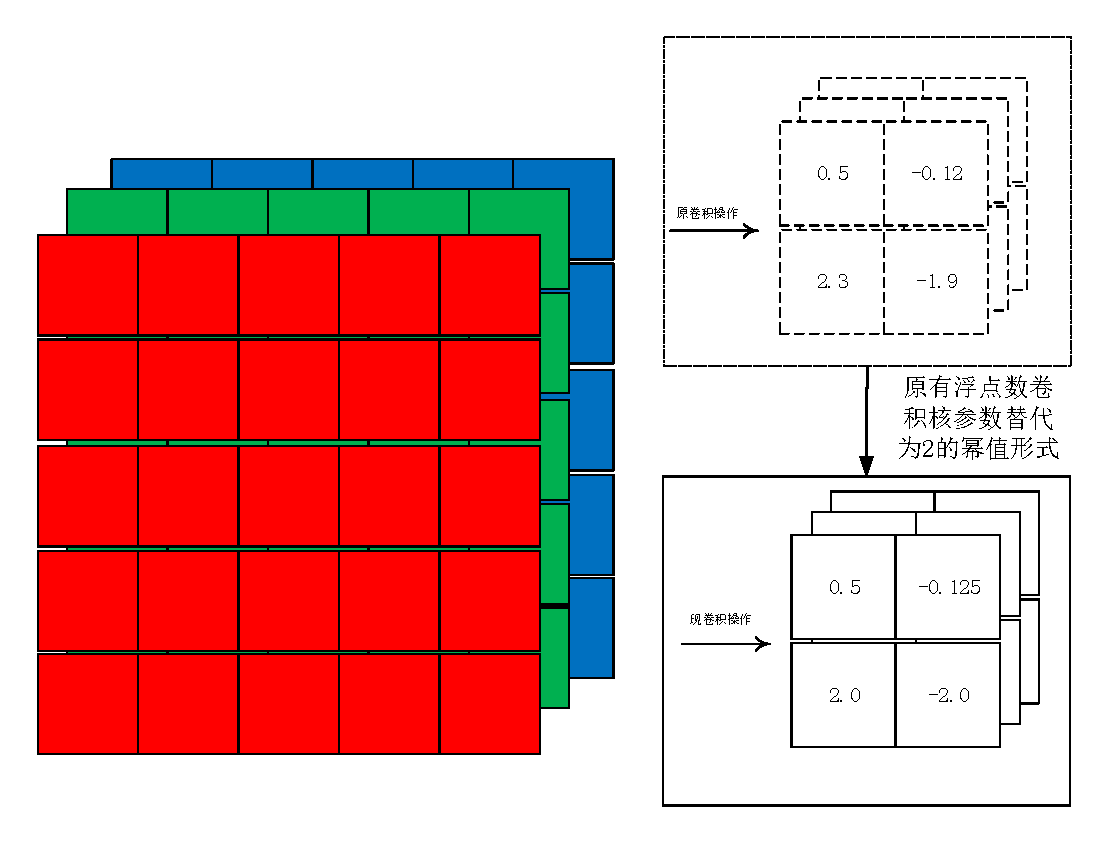
\includegraphics[width=0.7\linewidth]{quantization.pdf}  %插入的图,包括JPG,PNG,PDF,EPS等,放在源文件目录下
	\caption{量化算法的简单原理示意图:将浮点数参数替换为2的幂值}  %图片的名称
	\label{quantization}   %标签,用作引用
\end{figure}

早期的量化算法将精力集中在模型压缩上,\cite{earlycompression1}通过hash函数,使得CNN模型得以共享参数,实现了存储的优化。\cite{earlycompression2}这篇文章则将参数限定在特定取值上,因为整个网络的参数数值种类有限,所以只需要有限的bit位作为编码就能表示出所有的参数。但是\cite{earlycompression1},\cite{earlycompression2}这两种方法在实际应用时,还需要将编码转化为实际数值,因此并不能起到对模型加速的效果。\cite{deepcompression}这篇文章也是较早提到量化操作的文章。该文量化操作之后,模型中的参数只是更稀疏,数值却是任意的浮点数,并不能对模型计算进行优化。\cite{binary1}这篇文章可以算是开了2的幂值作为模型参数量化目标的先河;这篇文章尝试将模型的参数以及各卷积层的输出都二值化为$\pm1$,但是最终在测试集上,二值化的模型的精度损失较大。为了提高网络的信息提取能力,\cite{ternary}中作者将网络参数范围放宽到了${-1,0,1}$,显然模型的精度比二值网络有所上升,但误差还是不可避免。

在此之后,研究者们开始分两个方向进行量化的研究。一派如\cite{binary}、\cite{xnornet}、\cite{qnn}、\cite{hwgqnet}、\cite{dorefanet:}尝试对网络计算量进行进一步压缩,这派研究者不仅努力将卷积的参数量化为$\pm1$或者$\pm2^n$,同时试图将卷积之后输出的特征图也进行量化为$\pm1$或者$\pm2^n$。如\cite{xnornet},作者尝试将参数,激活函数的输出值都量化为${0, \pm1}$,这种量化的好处是可以将卷积运算从浮点数乘法、加法变成xnor和bitcount计算。毫无疑问,\cite{xnornet}在计算量上的优化的十分有优势的,但是实验结果看来,这样的量化操作会造成模型分类精度的下降。部分研究者,如\cite{dorefanet:}、\cite{qnn}尝试放宽卷积输出特征图激活值的量化范围,研究者尝试将卷积中参数量化为$\pm1$,而激活值量化为$\pm2^n$.另一派仅仅尝试将参数量化,而不考虑对激活值进行量化,如\cite{ternary2}、\cite{incremental},其中\cite{incremental}是截止到目前为数不多能够保证模型分类精度不下降的量化算法。这篇文章的出发点和之前的量化工作都不太一样,作者并没有尝试训练出一个量化网络,而是训练了一个全精度的网络,然后将这个网络中的参数转化成了目标量化值。

在近两年对量化算法的研究,大致可以分三个主要方向。第一类研究追求模型存储、计算性能优化,依然尝试对网络参数甚至激活值进行二值、三值量化。\cite{icasspq74}中,作者根据设定好的阈值将模型转化为三值网络,主要创新点在于对学习率的调整、以及利用正则化项等方法让网络稀疏化。\cite{cvprq71}中作者尝试对预训练好的模型,利用张量展开技术,利用放缩(scale)后的二值filters来拟合原来全精度的filters。\cite{iccvq71}中,作者不仅尝试将网络参数二值化,还尝试将输入的图片二值化。很多量化工作都尝试将卷积层输出的激活值量化,但是该工作是第一个尝试将网络的输入图片进行二值化的。众所周知,二值化、三值化的网络在分类精度上会有较大的损失,\cite{nipsq71}中,作者提出了用多组二值filters的加权来拟合同一个全精度filters,存储和计算优化效果比不上纯粹的二值化网络,但二值化后模型分类精度更有优势。\cite{cvprq84}中作者提出了基于梯度的对称量化方法,结合放缩技术对网络进行二值化。\cite{eccvq84}是\cite{xnornet}的一个升级版本,在参数量化上,这篇文章并没有太多新意,主要创新在于训练时对梯度计算进行了一定的优化,如对符号函数的求导进行近似。

第二类研究考虑道模型精度、算法落地的问题,尝试将神经网络参数低比特量化。这类工作中,算法的量化目标值是非特殊的,如2的幂值形式,因此往往更关注量化算法对模型的压缩效果。\cite{icasspq71}中作者利用对数编码,对非均匀分布的模型参数进行编码。\cite{icasspq72}将模型参数量化为定点数,最大的创新点在于量化操作后重新训练模型参数时,动态估计量化操作的步长。\cite{icmlq71}和\cite{icmlq72}都尝试将模型量化为低比特位数的参数,其中\cite{icmlq72}中更进一步给出了模型精度的证明。大量的量化算法工作都关注模型在推断(应用)阶段的数值量化,\cite{iclrq81}提出了一种新的方法,在训练阶段和模型的应用阶段都能实现了模型参数精度的降低为低比特位的整数。同时\cite{iclrq81}尝试将正则化层的计算转化为常数放缩,极大优化了模型的计算消耗。\cite{iclrq82}将模型参数、激活值以及梯度量化为半精度,同时在训练过程中,引入了对半精度梯度的放缩、单精度参数暂存的操作,保证了模型的训练精度。\cite{cvprq82}中,模型参数被量化为整数,虽然模型压缩幅度不高,但是这篇文章提出了一些有益的观点,如量化算法应该在更轻量的模型上测试,这篇文章的实验基于MobileNet,并在硬件上进行了测试。传统量化算法往往将参数和激活值一同量化,而\cite{cvprq86}中,作者先优化网络的权重量化值,然后在量化激活值,实现了更好的量化效果。\cite{eccvq81}中引入了强化学习算法来指导压缩,实现了更好的压缩效果。\cite{eccvq86}这篇工作中,作者研究了权重、激活值的数值分布情况,根据分布确定参数、激活值的量化范围,实现了较好的量化效果。

第三类研究开始考虑模型的训练代价。一部份工作,开始尝试将模型训练过程中的梯度低比特化。现有的深度学习模型面对越来越大的数据集,往往需要分布式的集群来实现模型训练,而分布式集群中CPU、GPU之间的信息传递往往需要较大的通信代价。因此如果能将模型的梯度量化为低比特形式,那么模型训练过程中的通信代价会小很多,实现对模型训练的加速。\cite{nipsq72}中作者关注于分布式深度学习模型训练中通讯代价的问题,提出了TernGrad机制,分布式之间传递三值的梯度,并基于对梯度值范围的假设,给出了理论证明。\cite{icmlq83}也是对深度学习模型并行化训练通信代价的优化:将传递中的局部梯度,量化为低比特位的梯度,优化通信代价,提升训练效率。除了模型并行化时训练代价的优化,\cite{nipsq75}中作者提出了对反向传播计算梯度时的存储量的优化。现有的深度学习模型在训练过程中,为了便于反向传播计算梯度,往往需要存储各卷积层的激活值。\cite{nipsq75}中作者基于ResNet进行了改进,提出了Reversible Residual Network(RevNet),在模型训练过程中不需要存储激活值,优化了训练模型阶段的存储消耗。

还有学者对量化算法的理论进行了一定的研究。如\cite{nipsq74}回顾了各种量化算法,从理论视角解读各类量化算法,研究各种训练量化网络的方法的差异。作者基于凸的假设,研究了训练算法精度的保证。基于问题非凸的假设,作者发现高精度参数的网络执行的是贪心搜索,而量化的网络缺乏这一过程。这从理论上解释了为什么低精度量化算法训练的困难。

\subsection{剪枝算法}
剪枝算法有着很悠久的历史,早在1990年前后,已经有研究者开始尝试将剪枝算法应用于神经网络\cite{90prune}、\cite{92prune}。早期的剪枝算法主要集中于对模型参数的剪枝,这样的剪枝不仅可以优化模型的存储大小,同时还可以起到防止模型过拟合的效果。总得来说,剪枝算法就是利用某种标准将模型中不重要的参数或者filters选出,然后剪掉,从而在保证模型精度的同时,尽可能压缩模型的存储空间、计算消耗。

截止到今天,CNN模型的剪枝算法大致可以分为两类:第一类以模型的参数修剪作为目标;第二类则以模型的filters(或者说通道数channels)作为剪枝目标。图 \ref{pruning_contrast}中简略地展示了两类剪枝的大致原理。参数剪枝算法,着重修剪参数,让卷积核变得稀疏,这样模型需要存储的参数数量会变少,从而能起到对模型存储进行压缩的效果。但是在参数剪枝算法中,卷积核变得稀疏,但是卷积核本身的数量并没有变化。这类剪枝算法在2016年之前比较流行,如\cite{9}中作者根据参数数值判断参数的重要性,改方法被结合到经典文章\cite{10}。在\cite{12},\cite{16}中,作者结合Lasso思想,借用惩罚函数构造稀疏卷积核。但是不管是怎样的标准,总不可避免会过度剪枝,因此在\cite{11}中作者提出了一种动态剪枝技术,通过标准来恢复部分参数。 稀疏卷积核的卷积操作需要依赖特定的库,所以实际上对CNN的卷积操作加速效果并不理想。
在16年之后,研究者们改变思路,不再以参数作为剪枝目标,而是开始剪filters。如图 \ref{pruning_contrast}展示了修剪filters的示意图,对filters的剪枝改变了卷积层输出的特征图数。

\begin{figure}[h]
	\centering
	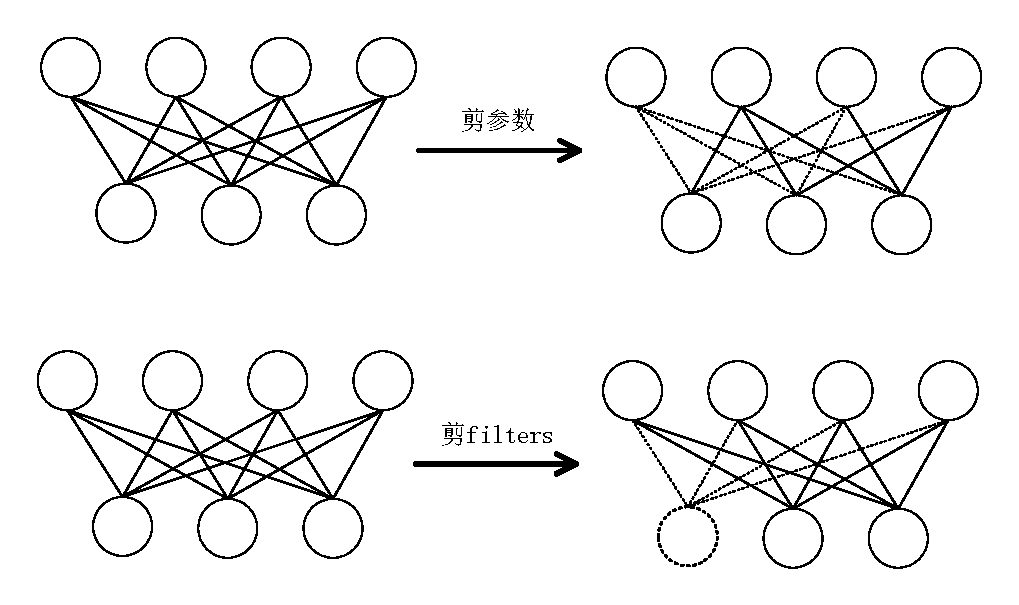
\includegraphics[width=0.7\linewidth]{pruning_simple_contrast.pdf}  %插入的图,包括JPG,PNG,PDF,EPS等,放在源文件目录下
	\caption{两类剪枝算法的对比:参数剪枝和filters(channels通道)剪枝.图中虚线部分代表被剪去的参数;圆代表被剪去的filters(channels)}  %图片的名称
	\label{pruning_contrast}   %标签,用作引用
\end{figure}

在剪枝filters的工作中,相当多的作者都在努力探索更优的标准来实现更好的剪枝效果。17年的\cite{17},作者使用filters的$l1-norm$来度量filters的重要性,范数值越大的filters越重要,剪枝时优先将不重要的filters剪去。\cite{18}中,作者使用紧跟着卷积层的BatchNorm层的放缩因子$\gamma$来度量filters或者说通道(channels)的重要性,$\gamma$数值越小相应的filters越不重要。\cite{21}提出了利用泰勒展开式来度量filters重要性。也有工作不仅关注模型压缩,更关心模型的计算量优化:\cite{energy}中,作者根据各个filters的计算量进行了排序,优先剪去计算代价大的filters。

近两年的剪枝领域的研究者们,一部分还注重对剪枝标准的发掘。如\cite{cvprp71},这篇文章中作者根据各个卷积层中不同filters消耗的能量代价进行抉择,优先减去能量消耗大的filters。\cite{icasspq73}中作者利用Group Lasso regularizer来判别filters的重要性。\cite{nipsq73}中作者引入了贝叶斯的观点,利用先验知识来来进行剪枝。\cite{icmlq81}中,作者利用信息瓶颈理论来指导剪枝。\cite{nipsp73}提出的想法比较有趣,作者并不会剪出一个固定的“瘦”的网络,而是将剪枝过程建模为马尔可夫决策过程,并利用强化学习算法进行决策。在模型对图片进行预测时,进行动态剪枝。

另一部分研究者则开始了训练稀疏模型的研究。如\cite{icmlp71}和\cite{iclrp81}中,作者利基于范数的正则化项,以及卷积层输出的特征之间的正负相关性,实现网络的稀疏化。\cite{cvprp81}除了考虑构建稀疏化的网络,更考虑了不同网络层,稀疏化的比例系数。\cite{iccvp71}中作者基于LASSO regression进行重要filters的选择,之后利用最小二乘法重构网络。

除了提出各种标准来判断filters的重要性或者构建稀疏化网络,还有一些研究者尝试利用现有的模型、算法搜索CNN网络内在的有效结构。\cite{28}和\cite{iclrp82}中作者利用LSTM提取模型中的有效结构。\cite{29}通过简化CNN网络计算图实现了对CNN网络结构的优化。

也有部分研究者将量化起来和剪枝算法结合起来,如\cite{nipsq73},\cite{iclrq82}和\cite{icmlq83}。

\section{待研究的问题}

\subsection{量化算法目标值集合的优化}

在所有量化算法中,近年的量化算法更着重于对模型计算量的优化。通过将参数优化为量化目标值$\{0,\pm2^{n_1}, \pm2^{n_2}, \pm2^{n_3}, \dots\}$,这样不仅能优化存储量,还想优化计算。但是在量化目标值的选择上,现有的算法并没有给出很好的解决方案。如\cite{binary}、\cite{ternary}等文章人工指定了量化目标值为0或者$\pm1$;而类似\cite{incremental}根据参数最大值,以及量化参数比特位数,确定了连续的量化目标值范围$\{0,\pm2^{n_1}, \pm2^{n_2}, \pm2^{n_3}, \dots\}$,其中$n_1$、$n_2$、$n_3$为连续的整数。现有的量化算法,只有很少的研究考虑对量化目标值集合的优化,这类研究通常是根据分布优化量化目标值集合。如\cite{icasspq71}中作者根据卷积网络参数的分布进行对数编码;\cite{eccvq86}同样也是根据分布确定量化目标值,但是这篇工作中量化目标值是非2的幂值形式的,不能起到优化计算速度的作用。\cite{eccvq87}中作者考虑的不再是根据模型参数分布确定量化目标值,而是根据卷积层输入数据的分布,来考虑量化目标值集合的确定。

本文第一部分工作尝试根据卷积层的参数数值分布,生成更好的量化目标值集合。该想法中首先定义了量化函数、量化操作的误差函数,为了最小化量化操作的误差,我们利用聚类算法生成量化目标值集合。最终的实验结果证明,优化之后的量化目标值集合有更好的性能。通过对量化目标值集合的优化,利用相同的量化算法,可以实现对现有CNN网络更大幅度的压缩。

\subsection{量化目标值集合应用范围的调整}

现有的量化算法量化目标值的应用范围大致为两种:1.整个网络,如\cite{binary}、\cite{ternary}是将整个网络所有参数优化都优化为$\pm1$;2.整个卷积层\cite{incremental}中每个卷积层都被量化到同一个目标值集合中。但是目前大多数量化算法的研究者们从没有明确提出量化目标值集合应用范围这一概念,也没有主动考虑在应用范围上进行研究。\cite{cvprq71}提出了基于filter的想法,但是并没有根据filters生成量化目标值,而是选择了基于filters对二值化网络进行不同比例的放缩,且该算法依赖于与训练好的深度学习模型。

本文的第二个工作明确提出了量化目标值集合应用范围的概念。设计了一种不依赖于预训练网络,直接训练二值化网络的算法。实验中,我们选定了以filters作为量化目标值集合的应用范围,针对不同的filters生成各自不同的量化目标值集合,之后基于相同的二值化的算法,测试了这种基于filters生成量化目标值的思想。实验结果证明,同样是二值化网络,通过对filters中参数分布生成各自的量化目标值集合,能有效提升二值化网络的分类精度。

\subsection{剪枝算法预训练量的思考}

现有的对filters的剪枝算法大致可以分为两类,一类是基于某种标准对预训练的网络进行迭代剪枝,第二类则是训练一个稀疏化的网络。第二类训练稀疏化网络的算法,我们认为可以看作是在训练过程中不断地进行剪枝,直到网络最后收敛。

对于第一类剪枝算法,剪枝过程很依赖预训练好的模型。而预训练过程往往需要数百个epochs。但是基于大量的预训练周期,得到的剪枝决策往往还是不够高效果的——不能只用一次剪枝操作就对CNN网络完成较高比例的剪枝。所以几乎所有的第一类剪枝算法,都有一个迭代剪枝的过程。

既然大量预训练无法让现有的剪枝算法得到高效的剪枝决策,那么剪枝操作之前大量的预训练未必是必须的。基于这种思想,本文中提出了基于少量预训练的剪枝思想。并基于现有的剪枝策略,测试了这种思想的有效性。实验结果证明,现有剪枝算法中,至少有一部分算法基于少量的预训练和基于大量预训练之后取得的剪枝效果不相上下,甚至有时候基于少量预训练的剪枝性能会更好。

必须强调,我们的方法是完全不同于第二类的稀疏化训练思想的。一方面,我们这里提出的基于少量预训练的剪枝思想,是对传统基于标准剪枝算法预训练量的思考,使用的剪枝标准可以是任何第一类的剪枝算法的剪枝标准;另一方面稀疏化剪枝算法需要在模型训练过程中持续剪枝到最终网络收敛,而我们的方法在网络训练过程中,并不需要持续剪枝,对于模型训练阶段的计算量优化效果更好。


\chapter{相关知识}
本文的工作都是关于深度学习模型压缩、加速技术的。现有的压缩、加速算法都集中在对计算量最大的卷积操作的改进,所以在本段中首先会重点介绍卷积神经网络(CNN)的卷积操作。为了便于读者构建对CNN基本认知,同时本文也会顺带简单介绍CNN中的常用技术。本文第一项工作是对现有量化算法的量化目标值集合的优化。该优化是利用参数分布来优化量化函数的目标值,这里利用了聚类算法,因此会在本段第二部分中简单介绍一下聚类算法。


%本文的工作集中在对CNN网络的量化和剪枝上,因此下面也尝试更细节上说明

\section{深度CNN常见技术}
CNN网络主要被应用于图像处理领域,常用的技术有卷积层(Convolution Layer)、激活函数、批标准化Batch Normalization \cite{batchnormalization},dropout \cite{dropout1},\cite{dropout2},池化层\cite{networkinnetwork}和全连接层。一般卷积层和激活层被用来提取图像特征,而全连接层则用来根据提取出来的特征进行分类。而深度CNN网络相较于早期的CNN网络,主要特点就是层数更多,整个网络结构更深。下面主要介绍卷积层。

\subsection{卷积操作}
CNN网络的卷积层主要被用于提取图像的特征,因此卷积层的输入是图像,而输出的提取出的特征也是以图像的形式存在。在图 \ref{convolution}中展示了卷积操作的基本流程。图 \ref{convolution}中展示了一个输入为RGB图像的CNN网络,第一层的情况。每个卷积层(Convolution Layer)都由多个filters组成,每个filter都会对该层输入的所有特征图进行卷积,一个filter卷积完该层所有输入特征图后会输出一个特征图。通常,每个卷积层都会由多个filters构成。图中的虚线指明了卷积和图像中像素点的对应点乘关系。

\begin{figure}[h]
	\centering
	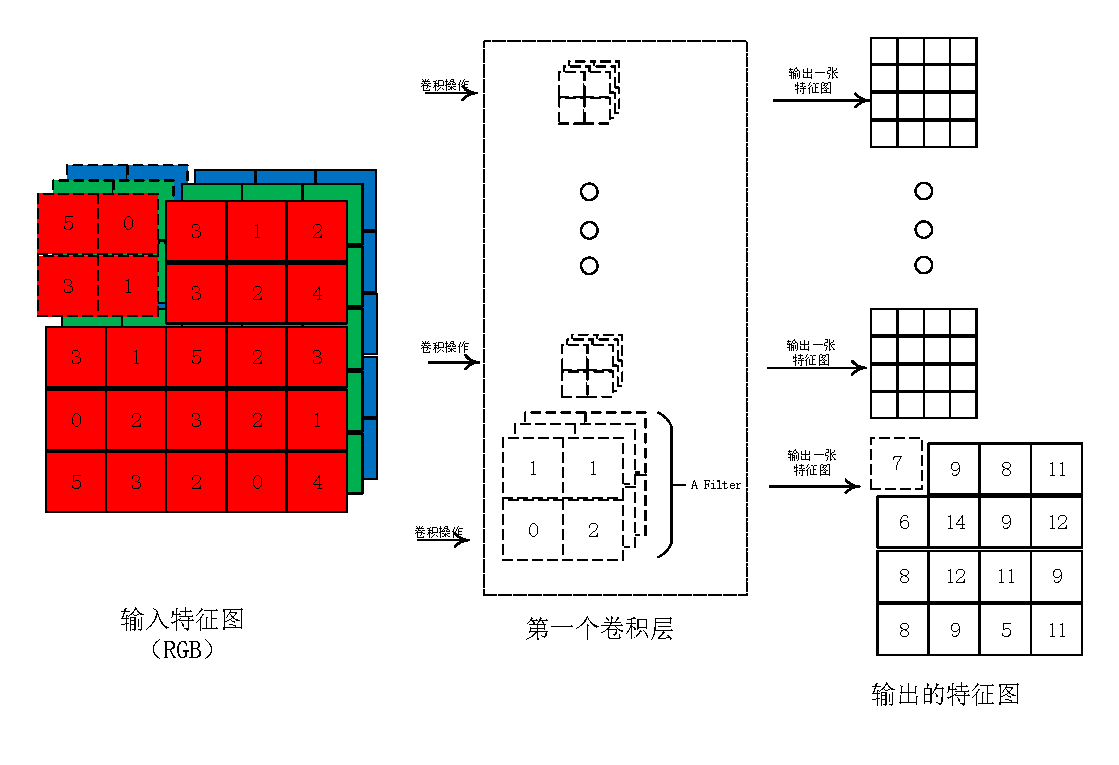
\includegraphics[width=0.7\linewidth]{convolution.pdf}  %插入的图,包括JPG,PNG,PDF,EPS等,放在源文件目录下
	\caption{卷积操作示意图}  %图片的名称
	\label{convolution}   %标签,用作引用
\end{figure}

\subsection{其他常见CNN网络技术}
CNN网络中常见的技术,还有激活函数、池化(pooling)、批标准化(Batch Normalization)\cite{batchnormalization}。现在通常在构建深度CNN网络时会将卷积层的输出进行正态标准化处理,同时约束网络、在训练过程中自动调整该标准化的强度,从而加快训练速度并降低权值初始化的成本。
激活函数已经成为神经网络的标配。如果没有激活函数,那么神经网络的输入到输出只是一个线性映射,而利用激活函数之后,可以神经网络可以学到更复杂的映射。在下图 \ref{activation}中画出了常见的四类激活函数。激活函数一般需要满足四个性质:可微性(便于计算梯度),单调性(保证函数是凸的),非线性(保证数据非线性可分)以及输出值范围有限。\ref{activation}中的Sigmoid和Tanh函数在输入值趋向$\pm\infty$时,函数梯度趋向于0,这在利用反向传播算法\cite{bp}计算梯度时,造成了梯度消失的问题。因此有研究者提出了激活函数\cite{relu},Relu作为激活函数输入为正时,梯度处处为1,极大缓解了梯度消失的问题。但是Relu函数对负的输入值求梯度时,梯度为0,这很容易造成神经元的“死亡”,梯度不能很好地回传,因此又有研究者提出了\cite{leakyrelu}.

\begin{figure}[h]
	\centering
	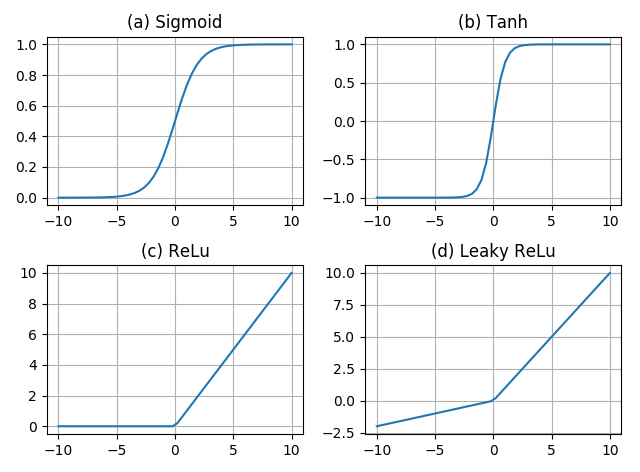
\includegraphics[width=0.7\linewidth]{activation.png}  %插入的图,包括JPG,PNG,PDF,EPS等,放在源文件目录下
	\caption{四种常见的激活函数}  %图片的名称
	\label{activation}   %标签,用作引用
\end{figure}

一般在卷积时,会使用paading(在图像周围补0)技术,用来防止卷积造成输出特征图尺寸变小。这样造成了数据维度的提升,为了降低数据维度,研究者提出了池化(pooling)技术。图  \ref{pooling}中展示了两种池化技术,池化技术会将图像的临近区域进行合并,合并值会选择区域内最大值(max pooling)或者区域内数值的均值(average pooling)。

\begin{figure}[h]
	\centering
	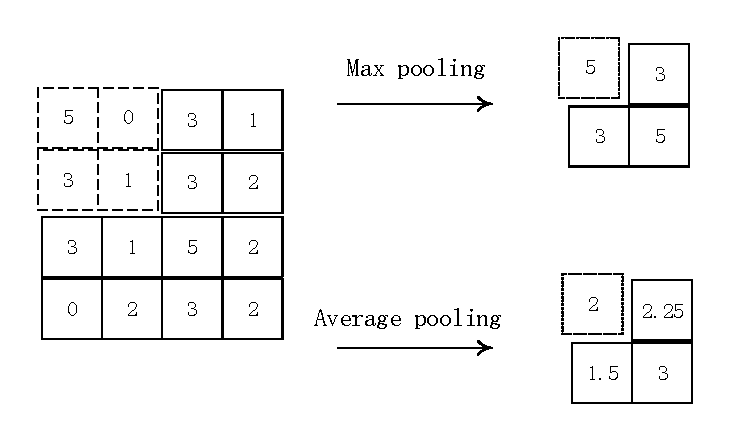
\includegraphics[width=0.7\linewidth]{pooling.pdf}  %插入的图,包括JPG,PNG,PDF,EPS等,放在源文件目录下
	\caption{两种池化技术:max pooling和average pooling}  %图片的名称
	\label{pooling}   %标签,用作引用
\end{figure}

一般来说,深度CNN网络中,一般卷积层、批标准化层、激活层是结合在一起使用的。

\section{聚类(Clustering)技术}
数据聚类技术属于无监督学习的一种。聚类算法会根据一定的标准将数据划分到不同的类别中去。聚类最终期望统一类别内的数据在特性上尽可能的接近;不同类别之间数据特性差异尽可能得大。
常见的聚类算法有很多种,有基于划分的,如经典的k-means算法;也有基于层次的,如BIRCH算法、CURE算法等;还有基于密度的算法,如DBSCAN算法。
本文应用聚类算法是为了大致探寻一维数据的分布。为了算法最终实现的简便,实验中选择的是最经典的k-means算法。k-means算法的大致流程如Alg.\ref{cluster}所示。
经典的k-means聚类算法需要设定超参数k,k对应聚类算法最终类簇的数量。开始进行聚类时,会首先随机选择k个数据点作为k个类簇的中心,然后利用欧式距离,将所有的数据点归类到这k个类簇中。接着在下一步中,算法会求出各个类簇内所有点的几何中心,作为新的类簇中心。之后进行下一轮迭代,直到类簇内数据点基本不再变动或者达到最大的聚类轮次,并输出聚类结果。


\begin{algorithm}
	\renewcommand{\algorithmicrequire}{\textbf{Input:}}
	\renewcommand{\algorithmicensure}{\textbf{Output:}}
	\caption{聚类算法流程}
	\label{cluster}
	\begin{algorithmic}[1]
		\REQUIRE 样本集$D=\{x_1,x_2,\dots,x_m\}$,聚类的簇数k,最大迭代次数N,
		\ENSURE 簇划分$C=\{C_1,C_2,\dots,C_k\}$
		\STATE 从数据集D中随机选择k个样本作为初始的k个质心向量: $\{μ_1,μ_2,\dots,μ_k\}$
		\STATE 对于 i = 1, 2, ${\ldots}$, N, 执行以下操作:
		\STATE \qquad 将簇划分C初始化为$C_t=\varnothing,t=1,2,\dots,k$;
		\STATE \qquad 对于$i=1,2,\dots,m$,计算样本$x_i$和各个质心向量$μ_j(j=1,2,\dots, k)$的距离:$d_{i,j}=\left\|x_i-μ_j\right\|_2^2$,将$x_i$标记最小的为$d_{i,j}$所对应的类别$λ_i$。此时更新$C_{λ_i}=C_{λ_i}∪{x_i}$
		\STATE \qquad 对于j=1,2,...,k,对$C_j$中所有的样本点重新计算新的质心$μ_j=\frac{1}{|C_j|}\sum_{x \in C_j}x$
		\STATE \qquad 如果所有的k个质心向量都没有发生变化,则跳出循环;
		\STATE 输出簇划分$C={C_1, C_2, \dots, C_k}$.
	\end{algorithmic}
\end{algorithm}


\section{算法验证数据集、模型的选择}

\subsection{数据集介绍}
图像分类领域,比较著名的数据集有MNIST\cite{lenet},MNIST-FASHION,SVHN,CIAFR10\cite{cifar},CIFAR100 和ImageNet\cite{alexnet}。这五个数据集是现行图像分类问题常用的验证数据集。MNSIT和MNIST-FASHION数据集共有十个类别,共由50000张训练集和10000张测试集组成,每个类别6000张图片。其中每张图片均为28*28。SVHN、CIFAR10和MINST数据集的类别、类内图片数量相同,不同的是SVHN和CIAF10数据集中每张图片大小为32*32。CIFAR100数据集和CIFAR10有相同的图片总数和图片大小,但CIFAR100中图片共有100个类别,所以每个类别有600张图片。这600张图片中,500张用作训练,100张作为测试。ImageNet数据集共有2万多个类别,一般实验中会选择其中的1000个类别来作验证。ImageNet每个类别有数百张图片,每张图片大小大约为256×256。
一般作者会根据自身的需求选择其中的一个、两个或者全部作为验证数据集。如\cite{17}选择了MNIST、CIFAR10数据集来作为验证集,\cite{28}选择了选择了MNIST、CIFAR10、CIFAR100作为验证数据集。\cite{27}中作者选择了CIFAR10和ImageNet作为验证数据集。

\subsection{算法模型介绍}
现有的比较经典的CNN模型有AlexNet,VGGNet和ResNet。因此现有的量化、剪枝算法一般会选择其中的一到两个模型来作为验证模型。如\cite{17}选择了VGGNet,ResNet验证模型,\cite{28}选择了VGGNet,ResNet作为验证模型;\cite{27}只选择了ResNet作为验证模型。
%AlexNet和VGGNet网络的原理基本相同,只是在结构上稍有区别;而在ResNe

\subsection{本文验证数据集和验证模型的选择}
现有数据集中,MNSIT,MNIST-FASHION,SVHN,CIFAR10数据集,数据集的图片数量适中,图片大小较小,所以选择了这两个数据集作为验证数据集。而ImageNet数据集规模过大,受限于硬件条件,本文放弃了该数据集。
验证模型的选择上,AlexNet,VGGNet和ResNet这三个模型均被采用。



\chapter{基于参数分布的量化算法目标值的优化}

\section{引言}
深度学习算法,在诸多领域取得了惊人的应用效果,这大大刺激了人们对深度学习的探索热情。但是深度学习模型高存储消耗、高计算量消耗也束缚着深度学习模型的更广泛应用。因此,对深度学习模型压缩、加速的研究逐渐引起了研究者们的兴趣。在所有深度学习模型中,CNN的压缩、加速一直是一大热点。近年来量化算法一直深受研究者们瞩目。
早期的量化算法,\cite{2014low}中,作者尝试利用低bit位数字来替代浮点数的网络参数,将浮点数运算简化为定点数运算。这样的操作可以使用更少的bit位来表示每个参数:之前每个参数都需要32bit来存储一个浮点数,现在是需要8bit甚至更少的bit位数来存一个定点数,整个网络存储消耗降低。同时还能优化计算代价,众所周知,在计算机上定点数计算比浮点数快得多。\cite{earlycompression2}中作者尝试性地将传统信息理论中的向量量化方法\cite{2011product}运用到了对CNN参数的优化上。

早期量化算法更多的将注意力集中在对模型的压缩上,近年的量化算法将注意力转向对卷积操作的计算量优化上。最开始研究者们尝试一步到位\cite{binary},将参数变为$\pm1$;之后的研究不仅想量化卷积核的参数,还想量化卷积核的输出特征图像素值\cite{binary1};由于参数量化过度,这类算法往往使模型在分类精度上损失较大。因此\cite{incremental}中,作者仅尝试将参数量化,取得了很好的量化效果。18年的\cite{extremely}通过量化算法和scale值的结合,利用ADMM算法,实现了很好的压缩效果。

近年的量化算法\cite{binary1},\cite{binary},\cite{ternary},\cite{incremental}中,研究者除了考虑模型存储压缩也在考虑优化CNN的计算量。这类量化算法的目标值通常是基于经验设定的,一般形式为${\{0,\pm1\}}$或者 ${\{0, \pm2^n\}}$。这类算法的量化目标值选择不够合理,通过优化量化目标值集合,现有量化算法可以在存储量上进一步被优化。在复现\cite{binary}算法的时候,我们发现,如果是用该算法处理原始CIFAR10数据集上的的AlexNet\cite{alexnet},会出现网络很难收敛的情况。虽然最终通过添加BatchNorm层这个问题被解决了,但是无疑证明如\cite{binary},\cite{ternary}在量化目标值的选择上,并不具有代表性。现有的工作往往都是根据经验、硬件需要指定量化目标值,本文提出了根据参数分布来确定量化目标值的办法。


\section{用聚类算法优化量化算法目标值}

\subsection{优化量化算法的目标值的意义} \label{sec1}

首先介绍两个概念:量化目标值和量化目标值集合。现有的量化算法,都会将CNN模型的参数转化为特定数值。如\cite{binary}中,最终CNN所有参数都被转化为1或者-1,那么这里的1或者-1就是量化操作的目标值,简称量化目标值。而一个量化算法在执行量化操作时,可以选择CNN中参数转化成某些值中的某一个,那么这些供选择的量化目标值的全集,即为量化目标值集合。在\cite{binary}中,量化目标值集合为$\{ -1, 1\}$,这意味着,最终量化完的CNN网络参数只能是1或者-1.

量化算法有两个作用:1.压缩模型存储;2.优化计算。现有量化算法的量化目标值集合通常为$\{0,\pm2^{n_1},\pm2^{n_2}, \pm2^{n_3}, \dots,\pm2^{n_k}\}$,其中k是一个超参,在计算优化上可以将浮点数乘法转化为bit位移运算。但是在压缩模型存储方面,现有工作尚有改进余地。

CNN网络的参数,往往以浮点数形式存在,量化算法的目标是使用某些数字取代浮点数参数,并同时想保证网络的精度。在量化目标值集合

$\{0,\pm2^{n_1},\pm2^{n_2}, \pm2^{n_3}, \dots,\pm2^{n_k}\}$

\noindent 中,k值越小,最终模型中的参数数值种类越少,实际存储中表示一个参数所需要的bit位数也越小。但是k值小到极限,那就网络就变成了\cite{ternary}网络,很显然过度的压缩模型参数取值范围会造成模型精度的较大损失。所以现有的量化算法不得不面对模型精度和模型存储之间的取舍。

现有算法在量化目标值的选择上是比较粗糙的。现有的量化算法如\cite{binary}、\cite{ternary}人为规定了量化算法的目标值为$\{0, \pm1\}$;\cite{incremental}中作者通过卷积层中参数的最大值和量化参数的bit位数要求确定量化目标值。其中\cite{incremental}是现有量化网络中为数不多能保证模型量化之后精度的算法。

现有的量化目标值集合,因为是人为设定或者基于经验,不能很好地代表其所要表示的参数。本文尝试选择更具有代表性的量化目标值集合,希望在保证精度的前提下,较之现有的量化目标值确定方法,能用更少的目标值表示网络,从而实现对CNN更高比例的压缩。本章实验通过卷积层参数的分布来确定量化算法的量化目标值集合。本章实验中将量化目标值集合相对于参数的代表性定义为一个优化问题。

首先假设量化目标值集合为$\{0,\pm2^{n_1},\pm2^{n_2}, \pm2^{n_3}, \dots,\pm2^{n_k}\}$,其中k值已经选定。之后本章定义了量化函数公式.\ref{formu:ori_quantization}:

\begin{eqnarray}\label{equ:ori_quantization}
\hat{W_l}(i,j)=\begin{cases}
2^{n_1}sgn(W_l(i,j))&\text{if $(\alpha+\beta)/2<abs(W_l(i,j))\leq3\beta/2$}\\
0&\text{otherwise},
\end{cases}\
\label{formu:ori_quantization}
\end{eqnarray}

上式中,α和 β是目标量化值中临近的两个值。 在进行量化操作的时候,本章会根据公式 \ref{formu:ori_quantization}将浮点数参数量化为目标值。根据公式.\ref{formu:ori_quantization},每个浮点数都会被量化为最接近该数的量化目标值,如$-0.12$会被量化为$-0.125$($-2^{-3}$)。

本文提出一个量化算法量化操作误差的度量公式 \ref{error_func}:

\begin{eqnarray}
min \sum_{l}\sum_{i,j}|W_l(i,j)-\hat{W_l}(i,j)|,
\label{error_func}
\end{eqnarray}

其中$W_l(i,j)$表示第l层的某个参数,$\hat{W_l}(i,j)$是该参数量化之后的数值。本章通过累加所有卷积层所有参数的量化误差,即可求出特定量化目标值集合的误差。当k值一定时,公式.\ref{error_func}值越小的量化目标集合越有效。考虑到该函数是个非凸函数,难以优化。本章考虑从CNN模型的参数分布来入手,选择量化算法的目标值。本章最终实验中选择了聚类算法来度量CNN网络的参数分布。

\subsection{使用聚类算法优化目标值的具体流程}\label{sec1.1}

在图 \ref{cluster_quantization}中对比了传统的量化目标值确定方法和本文方法的流程。如图 \ref{cluster_quantization}上半部分,现有的量化算法在确定量化值的时候并没有考虑参数的分布,如果想保证量化操作之后网络的精度,就需要更多的参数值。最终导致单个参数需要消耗更多的bit位来表示。而应用聚类算法之后,能够较好的发现各层网络的分布,从而挑选出更具有代表性的量化目标值。

\begin{figure}[h]
	\centering
	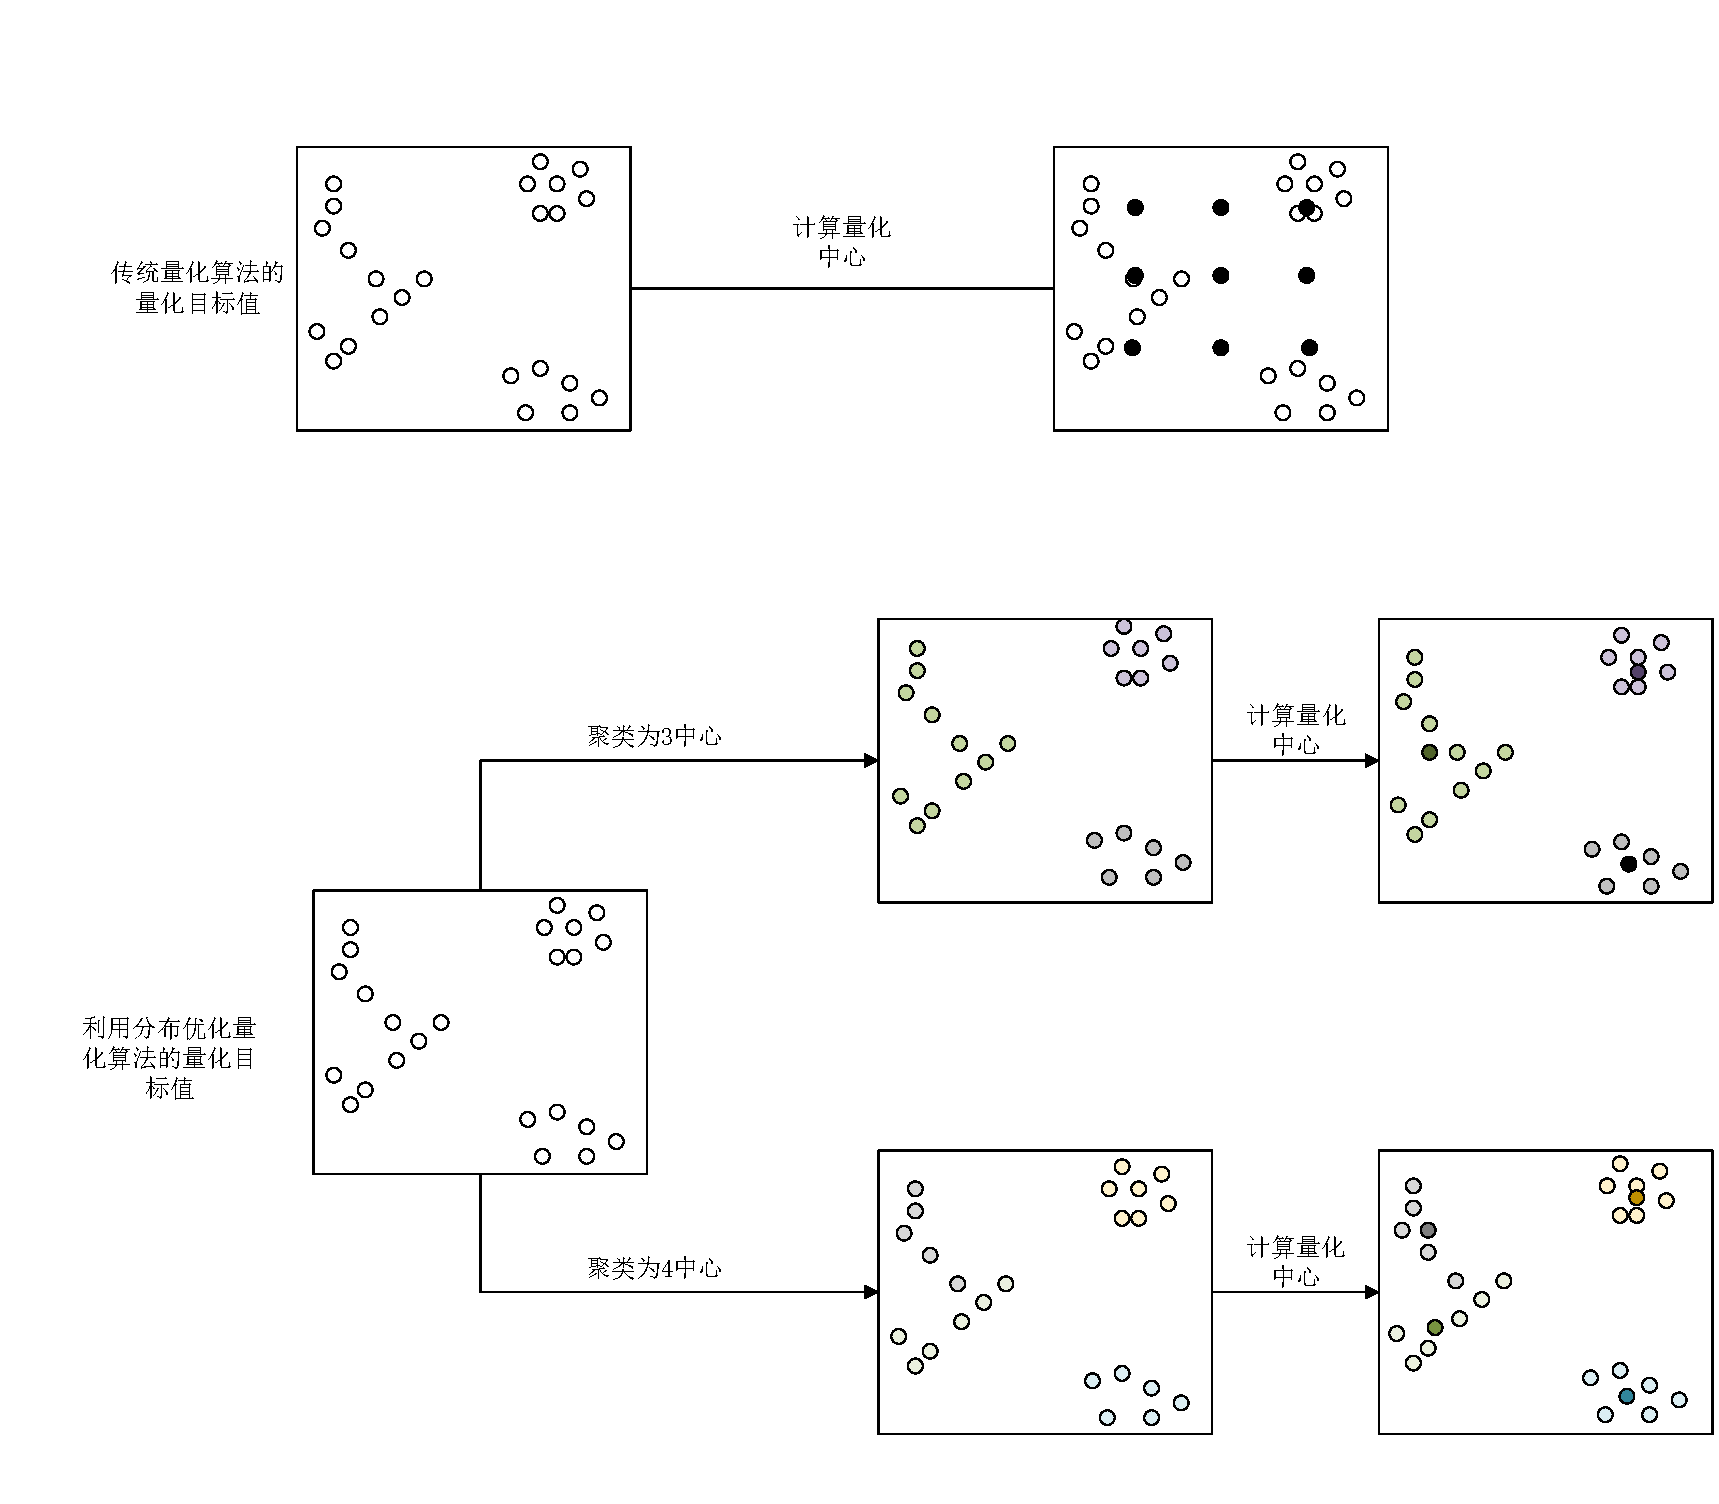
\includegraphics[width=0.7\linewidth]{cluster_quantization.pdf}  %插入的图,包括JPG,PNG,PDF,EPS等,放在源文件目录下
	\caption{传统方法和基于聚类的量化目标值集合的分布对比}  %图片的名称
	\label{cluster_quantization}   %标签,用作引用
\end{figure}

首先本章会设定超参数k,k是量化目标集合$\{0,\pm2^{n_1},\pm2^{n_2}, \pm2^{n_3}, \dots,\pm2^{n_k}\}$中的k,显然k值越小,最终存储参数时可以用更少的bit位表示,模型的压缩效果会越好。

假设CNN共有L层,那么用$Core_l=\{c_1, c_2, \dots, c_k\}$表示对第$l$层参数执行聚类算法得到的k个聚类中心。显然这k个聚类中心是浮点数形式的数字,并不能直接作为量化算法的目标值。因此还需要根据聚类中心,从$Quan_{set} = \{0,  \dots, \pm2^{-1}, \pm2^{0}, \pm2^{1}, \pm2^{2}, \dots \}$中选择合适的数字作为量化目标值。本章根据公式.\ref{quan3},将$Core_l$集合中的所有聚类中心转化为$Quan_l=\{\hat c_1, \hat c_2, \dots, \hat  c_k\}$

\begin{eqnarray}
\hat x = quan(x) = \gamma,
\gamma \in Quan_{set},
\forall y \in Quan_{set}, |\gamma - x|<= |y - x|,
\label{quan3}
\end{eqnarray}

通过公式 \ref{quan3},可以给CNN的每一个卷积层确定一组量化中心$Quan_l$。图 \ref{quan_fenbu}中展示了AlexNet网络中各卷积层参数的分布状况以及根据聚类求出的量化中心的分布。图中共有五幅图,每幅图对应AlexNet一层卷积。图 \ref{quan_fenbu}中用频数直方图统计各层的参数分布。通过观差直方图高度可以发现,各层的参数都以0为中心,绝对值越小的参数越多,绝对值越大的参数越少。图中黄线画出了传统量化算法量化目标值$\{0, \pm 2^n\}$的分布。红色的线表示的是通过聚类算法、得到的经过优化的量化中心。通过图像可以明显发现,通过聚类算法确定量化目标值集合,能使用更少的量化值就可以将CNN网络量化。

\begin{figure}[ht]
\centering
\begin{minipage}[t]{0.3\textwidth}
\centering
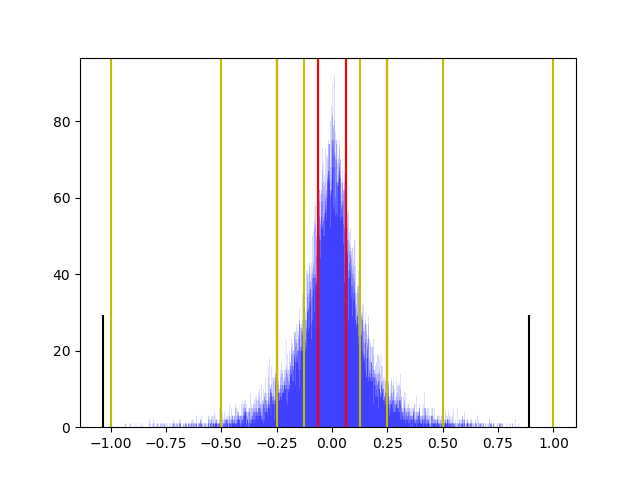
\includegraphics[width=1\textwidth]{11.png}
\end{minipage}
\begin{minipage}[t]{0.3\textwidth}
\centering
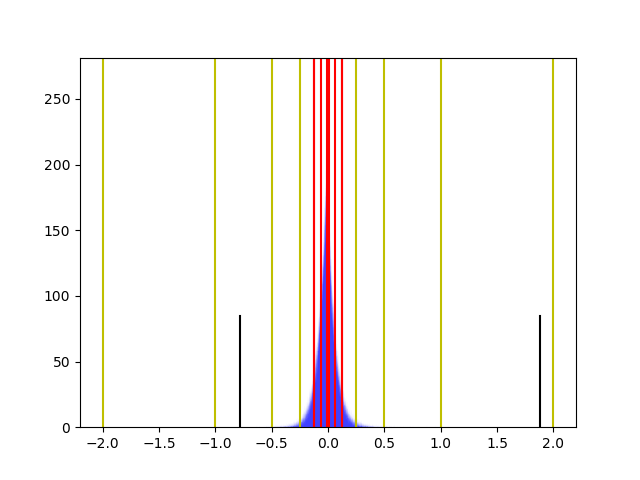
\includegraphics[width=1\textwidth]{12.png}
\end{minipage}
\begin{minipage}[t]{0.3\textwidth}
\centering
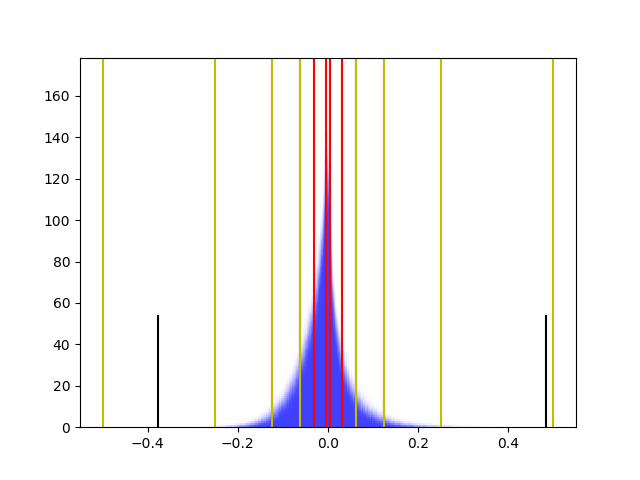
\includegraphics[width=1\textwidth]{13.png}
\end{minipage}


\begin{minipage}[t]{0.48\textwidth}
\centering
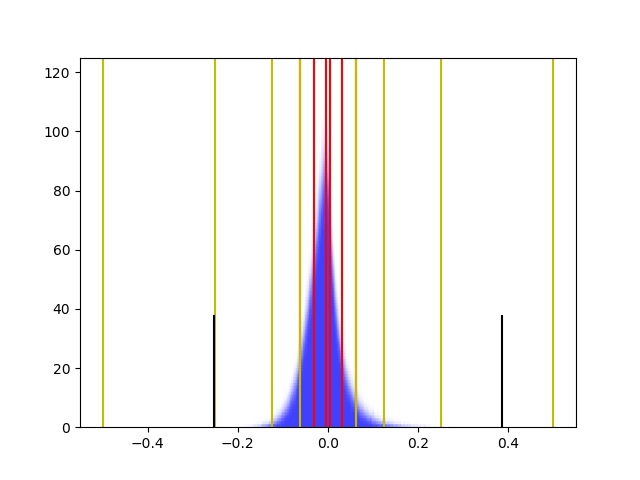
\includegraphics[width=1\textwidth]{14.png}
\end{minipage}
\begin{minipage}[t]{0.48\textwidth}
\centering
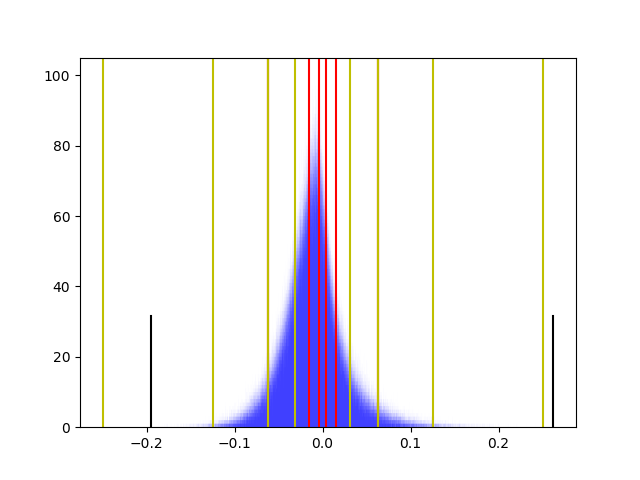
\includegraphics[width=1\textwidth]{15.png}
\end{minipage}
\caption{AlexNet中五个卷积层中参数的分布状况 }
\label{quan_fenbu}
\end{figure}


\subsection{实验算法流程}

目前现有的量化算法中,大部分算法在将CNN模型量化之后,都会造成精度上的损失。\cite{incremental}是目前所知为数不多能保证量化之后,模型精度不下降的算法。因此本章尝试优化\cite{incremental}算法的量化目标值。

\subsection{Incremental思想}

\cite{incremental}中,作者不同于之前的量化工作,并没有尝试将整个网络一次性全部量化为指定数值,而是尝试引入了Incremental的思想。首先作者设定了一个量化比例序列,如$\{50\%, 75,\%, 87.5\%, 100\%\}$。之后在执行量化算法的时候,是一个迭代过程,首先训练一个全精度的网络,然后根据量化函数,量化CNN各卷积层$50\%$的参数;之后是一个retraining的阶段,通过对模型未量化的参数进行训练,恢复量化操作之后模型的精度损失;然后按照$75\%$的比例量化更多的参数,再继续retraining剩下的参数;如此循环。在图 \ref{incremental}中,方块代表卷积核,卷积核中数值的变化过程展示了Incremental思想下的量化流程。

这幅图中,顺着箭头展示了Incremental量化算法的流程。图中彩色部分标明了待量化或者已被量化、并固定住数值(不再参与模型参数训练)的参数。白色部分标明了剩余的参与模型retraining的参数。图中每次量化操作都使用了一种不同的颜色标明本轮量化操作会量化的参数的位置。如前两幅中,第一幅图中的红色标出了方块的所有参数中最大的$50\%$的参数,这部分参数是待量化的;通过第二幅图可以发现经过量化操作,红色部分的参数已经被量化为$2^n$的形式;而且红色部分的参数在之后的retraining过程中,数值是不发生变化的。第三、四幅图中黄色部分标明了第二轮量化操作具体将哪些参数量化成了2的幂值形式。

\begin{figure}
\centering
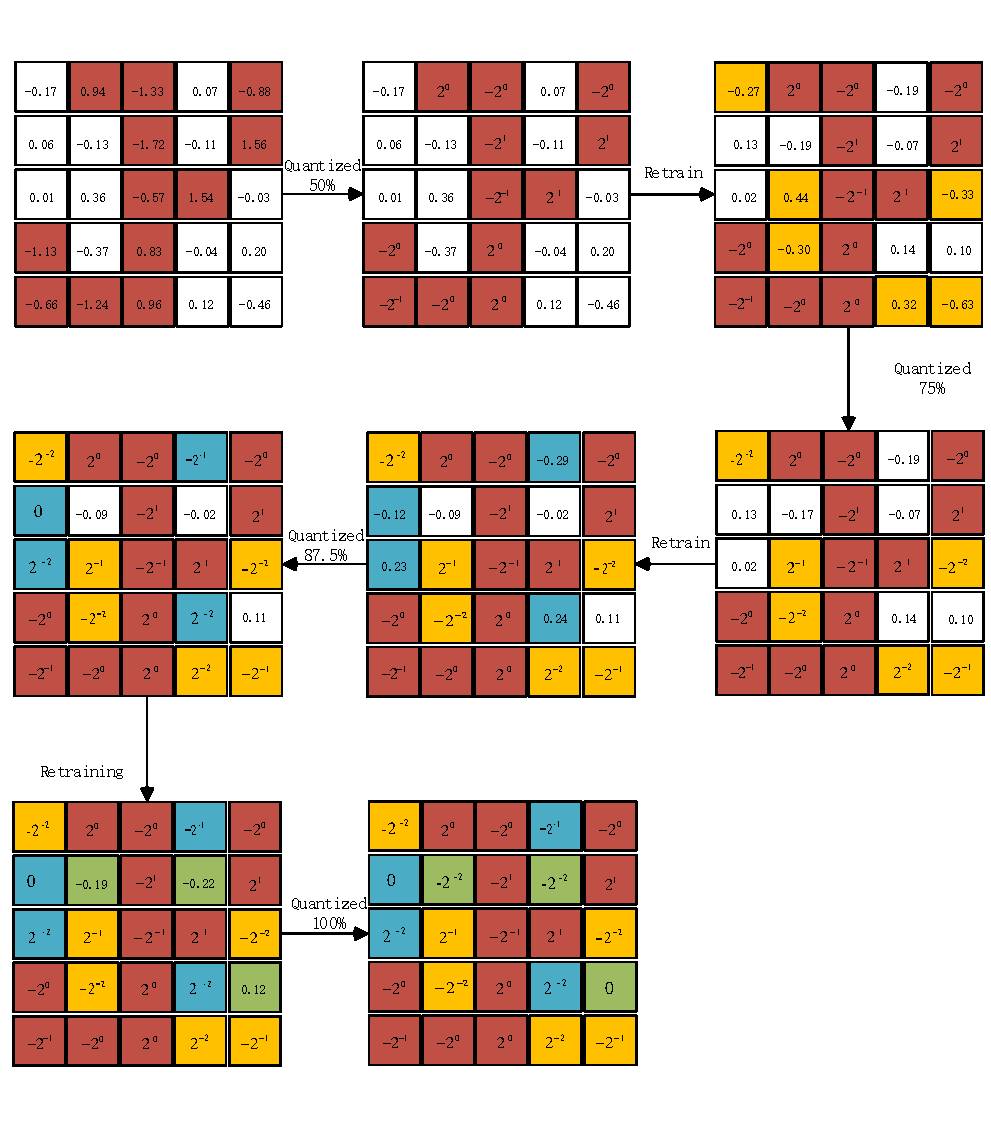
\includegraphics[width=0.85\textwidth]{incremental.pdf}
\caption{Incremental量化算法的流程}
\label{incremental}
\end{figure}

其中,假定根据第 \ref{sec1}章节中的聚类、量化流程,已经计算出了CNN各层的量化中心$Quan_l=\{\hat c_1, \hat c_2, \dots, \hat  c_k\}$。那么本章会根据公式 \ref{for:quantization}完成图 \ref{incremental}中对每个参数的量化操作。

\begin{eqnarray}
\hat{W_l}(i,j)=\begin{cases}
2^{n_1}sgn(W_l(i,j))&\text{if $\frac{2^{n_1}}{2}<abs(W_l(i,j))\leq\frac{2^{n_{1}}+2^{n_2}}{2}$}\\
2^{n_i}sgn(W_l(i,j))&
\text{if $\frac{2^{n_{i-1}}+2^{n_i}}{2}< abs(W_l(i,j))\leq \frac{2^{n_{i}}+2^{n_i+1}}{2},$}\\
&\text{$i=2,\ldots,k-1$}\\
2^{n_k}sgn(W_l(i,j))&\text{if $abs(W_l(i,j))>\frac{2^{n_{k-1}}+2^{n_k}}{2}$}\\
0&\text{otherwise},
\label{for:quantization}
\end{cases}\
\end{eqnarray}

\section{实验}

\subsection{实验设置}

本实验是在MNIST和CIFAR10数据上进行的。MNIST是一个关于手写数字的的数据集,每张图片均为黑白照片,大小为28*28像素。图 \ref{fig:mnist}是打印的一些MNIST数据集中手写数字的图像。在实际存储中,数据集中每张图片都是以矩阵形式存储的一个数阵,矩阵中每个数都对应实际图像中相应像素点的像素值。对于MNIST数据集而言,矩阵中的数值越大,则实际图片中该点的颜色越黑。为了便于文章的布局,CIFAR10数据集的详情会分到下一个工作中再做详细介绍。

\begin{figure}
\centering
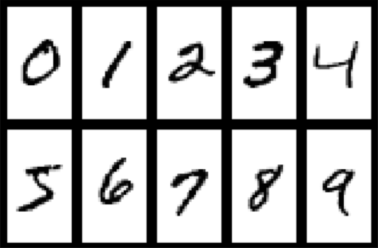
\includegraphics[width=0.7\textwidth]{mnist.png}
\caption{MNIST数据集中的图片}
\label{fig:mnist}
\end{figure}

在模型选择上,本章选择了一个普通的CNN网络,AlexNet以及VGGNet作为验证模型,来验证优化之后的量化中心的有效性。

\subsection{实验过程}

本部分工作主要共享在于对现有量化模型目标值的优化,希望能在同样模型分类精度下,用更少的数值表示模型参数,实现对模型存储的进一步压缩。本章选定了\cite{incremental}中的量化算法进行优化。所以对比实验主要在优化前后的增量式量化算法上。本章中使用聚类算法解决了公式 \ref{error_func}难以优化的问题。同时本章发现在\cite{18incre}中也有用到聚类算法,但在我们工作的思想和\cite{18incre}不同,本章的工作中聚类算法是用来解决公式 \ref{error_func}的优化问题的,更多的是将优化目标值集合的思想引入近年的量化工作中。最终在量化操作时,本章的实验基于参数数值划分实现起来也更简单。

第一组对比实验是基于MNIST数据集和一个普通的CNN网络。由于MNIST数据集比较简单,本章基于MNIST的实验并没有使用AlexNet、VGGNet等大型网络,而是随机设定了简单的CNN网络。可能是由于MNIST数据集复杂度较低,在实验时我们尝试更换了多种结构的CNN网络,实验结果都比较类似。最终实验结果是基于一个拥有4层卷积层的CNN。

首先,本章在MNIST数据集上训练了一个全精度的CNN网络,之后根据\cite{incremental}中的量化算法,确定该CNN各卷积层的量化目标集合为

\begin{eqnarray}
Quan_{l,old} = \{0, \pm2_{n1}, \pm2_{n2} , \dots, \pm2_{nk_0}  \}
\end{eqnarray}

\noindent 之后根据增量式的思想逐步将CNN中的参数量化为$Quan_l$中的值。

之后本章采取利用参数分布优化量化目标值的思路,优化各层的量化目标值集合,求出了新的$Quan_{l,new} = \{0, \pm2_{n1}, \pm2_{n2} , \dots, \pm2_{nk_1} \}$。为了保证量化目标值集合和原文\cite{incremental}中的一致性,在求新的目标值$Quan_{l,new}$之前,本章会先将所有参数绝对值化,然后求出聚类中心,进而求出$Quan_{l,new}$。具体流程如在第 \ref{sec1.1}章节中所述。

同样的实验流程,本章基于CIFAR10数据集,对AlexNet和VGGNet进行了一遍。

\subsection{对比方案}

原文\cite{incremental}中,量化算法并没有影响算法本身的分类精度。因此本章的对比试验中,不论优化前还是优化后,对比的前提是量化操作不影响网络的精度。在这一前提下,希望量化目标值越少越好,因为目标值越少,表示一个参数所需要的bit位数越少,量化算法对CNN模型的压缩效果越好。

本章中用$Quan_{l, old}$表示原文的量化目标值集合,$Quan_{l,new}$是利用基于聚类的优化方法得到的量化目标值集合。总结起来,如果$\left\| Quan_{l, new} \right\|_0$<$\left\| Quan_{l, old} \right\|_0$,则说明了基于聚类优化量化目标值集合的有效性。$\left\| Quan_{l, new} \right\|_0$比$\left\| Quan_{l, old} \right\|_0$数值上小的越多,证明基于聚类优化量化目标值的方法越有效。


\subsection{实验结果}

下面的表格展示了各项实验结果。

表 \ref{1mnist}和表 \ref{1cifar10}中,k指的是$Quan_{l} = \{0, \pm2_{n1}, \pm2_{n2} , \dots, \pm2_{nk} \}$中的k值。如k=2,即表明在量化目标值集合中$Quan_{l}$共有5个值,最终量化算法的目标值为$Quan_{l} = \{0, \pm2_{n1}, \pm2_{n2}$。k值反应了量化目标值的有效性,k值越小,且能保证模型的精度,那么量化算法目标值越有效。同时k值越小意味着参数的数值越少,表示同一个参数所需要的bit位数越少。总之,k值越小,模型压缩效果越好。

$ori_q(\%)$表示的是,原始的\cite{incremental}增量式量化算法量化模型之后,模型在相应数据集上的测试精度,单位为$\%$。$kmeans_q(\%)$表示量化的目标值经过聚类算法优化之后,对模型进形增量式量化,得到的模型测试精度,单位同样是$\%$。

表 \ref{1mnist}展示了普通CNN网络在MNIST数据集上的结果。实验中普通的CNN在MNIST数据集上,在未量化前,测试精度为$98.01\%$。通过表 \ref{1mnist}可以发现,当k取值为5时,不优化的量化目标值集合$Quan_{l, old}$还能保证增量式量化算法的有效性,但是当k值取为4时,$Quan_{l, old}$已经不能保证增量式量化算法的有效性了。而经过聚类优化的量化目标值集合$Quan_{l, new}$一直到k取值为3时都能保证\cite{incremental}增量式量化算法的有效性。


\begin{table}[tp]

  \centering
  %\fontsize{6.5}{8}\selectfont
  \caption{MNIST数据集上,普通CNN量化实验结果对比}
  \label{1mnist}
    \begin{tabular}{|c|c|c|}
    \hline
    \multirow{2}{*}{ }&
    \multicolumn{2}{c|}{$A CNN$}\cr\cline{2-3}
    &$ori_q(\%)$&$kmeans_q(\%)$\cr
    \hline
    \hline
    $k=2$&9.34&11.34\cr\hline
    $k=3$&10.94&97.30\cr\hline
    $k=4$&10.98&97.49\cr\hline
    $k=5$&97.29&98.03\cr\hline
    \end{tabular}
\end{table}

表 \ref{1cifar10}展示了AlexNet和VGG19网络在CIFAR10数据集上的优化结果。实验中训练出来的未量化的AlexNet网络在CIFAR10数据集上精度为$85.03\%$。通过表 \ref{1cifar10}可以发现,当k取值为8时,不优化的量化目标值$Quan_{l, old}$还能保证增量式量化算法的有效性,但是当k值取为7时,$Quan_{l, old}$已经不能保证增量式量化算法的有效性了。而经过聚类优化的量化目标值集合$Quan_{l, new}$一直到k取值为3时都能保证\cite{incremental}增量式量化算法的有效性。

表 \ref{1cifar10}可以看出,实验中训练出来的未量化的VGG19网络在CIFAR10数据集上精度为$94.13\%$。通过表 \ref{1cifar10}可以发现,当k取值为6时,不优化的量化目标值$Quan_{l, old}$还能保证增量式量化算法的有效性,但是当k值取为5时,$Quan_{l, old}$已经不能保证增量式量化算法的有效性了。而经过聚类优化的量化目标值集合$Quan_{l, new}$一直到k取值为3时都能保证\cite{incremental}增量式量化算法的有效性。

综上所述,经过聚类算法优化的量化目标值集合,只需要更少的数值就可以保证相同量化算法的有效性。可见通过参数分布,优化量化目标值集合$Quan_l$能实现对模型的进一步压缩。
\begin{table}[tp]

  \centering
  %\fontsize{6.5}{8}\selectfont
  \caption{CIFAR10数据集上,AlexNet和VGG19量化实验结果对比}
  \label{1cifar10}
    \begin{tabular}{|c|c|c|c|c|}
    \hline
    \multirow{2}{*}{ }&
    \multicolumn{2}{c|}{$AlexNet$}&\multicolumn{2}{c|}{$VGG19$}\cr\cline{2-5}
    &$ori_q(\%)$&$kmeans_q(\%)$&$ori_q(\%)$&$kmeans_q(\%)$\cr
    \hline
    \hline
    $k=3$&10.00&73.01&-&88.95\cr\hline
    $k=4$&10.00&74.10&10.00&89.03\cr\hline
    $k=5$&10.01&73.26&10.00&89.06\cr\hline
    $k=6$&10.00&73.58&89.70&89.12\cr\hline
    $k=7$&10.00&73.21&90.02&89.53\cr\hline
    $k=8$&73.33&73.93&89.13&89.76\cr\hline
    \end{tabular}
\end{table}


\section{本章小结}

本章尝试根据CNN网络的参数分布来为量化算法确定量化目标值集合。本章实验中,我们使用了相同的量化算法思路\cite{incremental}。从实验结果看,基于参数分布,利用聚类算法确定的量化目标值集合,能更用更少的数值表示出原CNN网络。因为量化目标值集合更小,所以表示每个参数需要的比特位更少,CNN网络也能被压缩得更小。我们的工作证明了,根据参数分布确定量化目标值集合是使用量化算法时,进一步压缩CNN存储的有效方法。


%#################################

%%%%%%
%%%%%%

%\chapter{关于量化算法量化目标值应用范围的思考}

%\chapter{基于filters确定的量化目标值集合}
\chapter{基于filters的量化算法目标值的优化}

\section{引言}

量化算法是现有的CNN模型存储压缩、计算加速算法之一。本节将先详细介绍量化算法对CNN模型的的存储压缩和计算加速的细节原理。

量化算法能对CNN模型的压缩原理。现有的深度学习框架中,训练出来的CNN模型参数都是浮点数形式的,假设是32位浮点数。那么CNN模型中每个参数都占32比特位数。假设某个CNN网络中共有$1,000,000$个参数,那么该CNN模型理论上的存储空间为32*1000000个比特,即32Mb或者说4MB。当参数为32位浮点数时,参数有三种范围:1.正浮点数,表示范围为$1.0*2^{-126} \approx 1.1755*10^{-38} \leq FloatNum \leq (2-2^{-23})*2^{127} \approx 3.4028*10^{38}$; 2.零浮点数,范围为0; 3.负浮点数,表示范围为$-(2-2^{-23})*2^{127} \approx -3.4028*10^{38} \leq FloatNum \leq -1.0*2^{-126} \approx -1.1755*10^{-38}$。可见,当参数为32位浮点数时,参数可取的数值范围是很大的。为了能压缩模型存储,量化算法考虑压缩每个参数的存储空间。不再用32位表示每个参数,尝试用8比特,甚至更少的比特位来表示一个参数。比如\cite{quantization}中,作者尝试用8比特的定点数取代32位浮点数来表示CNN中的参数。如果原网络有$1,000,000$个参数,32位浮点数构成的网络存储空间为4MB;如果将CNN网络中的32位浮点数全部替换为8bit的定点数,那么该网络的存储空间就压缩为1MB了;这样就实现了对CNN模型存储量的压缩。而在\cite{binary}中,作者尝试将所有的参数取值固定为$\{1, -1\}$。很显然将\cite{binary}中的量化算法将CNN网络量化之后,每个参数都只有两种取值,那么表示两种可能性只需要1比特即可。显然,\cite{binary}量化过的网络,每个参数都只需要1比特位来表示即可。如果该网络原有$1,000,000$个参数,原来模型占用的理论存储空间为4MB,现在只需要0.125MB即可。综上所述,在实现量化算法时,网络中参数的取值范围越小,对CNN模型的压缩比例越高,压缩效果越好。

量化算法能对CNN模型计算量优化。在计算机运算过程中,执行一次浮点数的加法(或减法、乘法、除法)运算比定点数同类型运算需要的指令周期数多,即浮点数运算要比定点数运算量消耗大,定点数运算会更快。而不论是定点数还是浮点数运算,在具体的指令周期中都会被拆解为位运算(bit operation)。可见一次位运算的计算量要比浮点数运算和定点数运算都少,速度更快。CNN网络主要的计算量就在于卷积层对输入特征图进行的卷积操作。卷积操作理论上主要是由浮点数乘除法组成。量化算法就是将CNN模型的参数或激活值转化为定点数或者2的幂值,这样就能将浮点数运算转化为定点数运算或者位运算。

目前的量化算法大致可以分为三类:第一类:\cite{quantization}将CNN网络中的参数和卷积层输出的激活值,都由浮点数都转化为定点数,那么CNN网络的卷积操作涉及的浮点数运算都将转化为定点数运算,卷积操作的计算量消耗更少,整个CNN网络的运算会更快;第二类:\cite{binary}、\cite{incremental}、\cite{extremely}等文章将卷积中的参数转化为$\pm 1$或者$2^n$的形式,那么卷积操作中的浮点数乘法将被转化为位移运算,从而起到了对CNN网络计算量优化的效果。本文要强调,在这类算法中,只有浮点数乘法会被转化为位移运算,但是因为卷积层输出的激活值并没有被量化,还是浮点数形式,这些浮点数需要加在一起构成输出特征图中的某个“像素点”。所以在这类量化算法量化之后的CNN模型中,浮点数加法依然存在;第三类:这类算法将量化思想发挥到了机制,代表作是\cite{xnornet}。这类量化算法将CNN网络中所有参数和激活值都转化为$\pm 1$或者$2^n$的形式。这样卷积操作中所有的浮点数运算都能转化为如位移、bitcount等位运算。这种方法能极大优化CNN网络的计算。虽然三类量化算法都能压缩模型存储空间,优化计算速度;但是将模型参数优化为$\pm 1$时,模型的精度还是有较大的损失。总之,量化算法对模型的加速依赖量化目标值的特殊——2的幂值形式。

现有的量化算法,通常都是整个网络或者同一个卷积层共用相同的目标量化值。如\cite{ternary}中,整个网络所有的参数,都会被量化为$\{-1, 0, 1\}$中的某个值,即整个网络都共用相同的量化目标值。\cite{incremental}则是各个卷积层共用量化目标值。假设量化目标值集合为$Set_{target} = \{t_1, t_2, \dots, t_n\}$,根据上文中量化算法压缩模型存储原理的说明,如果$Set_{target}$中的n值越小,最终模型存储的压缩比例越高。但是从\cite{binary}、\cite{ternary2}、\cite{xnornet}等文献中的实验结果来看,n值过小,CNN模型量化之后的分类精度又难以保证。

现有量化算法可以看作一个模型压缩比例和模型分类精度之间的权衡、取舍。本章针对这一取舍问题,提出了一个新颖的问题:能否在保证压缩比例的情况下,尽可能增加量化后CNN网络的分类精度?为了解决这一问题,本章提出了改变量化目标值集合$Set_{target}$应用范围的想法。

\section{量化目标值集合应用范围的相关概念 }

\subsection{量化目标值集合的应用范围}

量化算法的目标值集合$Set_{target}$指的是,CNN网络中参数被量化后的取值范围。如\cite{ternary}中,整个CNN网络参数都会转化为$Set_{target} = \{-1, 0, 1\}$中的某个值,那说明该量化目标值集合$Set_{target}$应用范围为整个CNN网络。而在\cite{incremental}中CNN网络第l个卷积层有自己的目标量化值集合$Set_{target,l} = \{t_{l,1}, t_{l,2}, \dots, t_{l,n}\}$。\cite{incremental}中每个量化目标值集合$Set_{target,l}$的应用范围为一个卷积层。

\begin{figure}
\centering
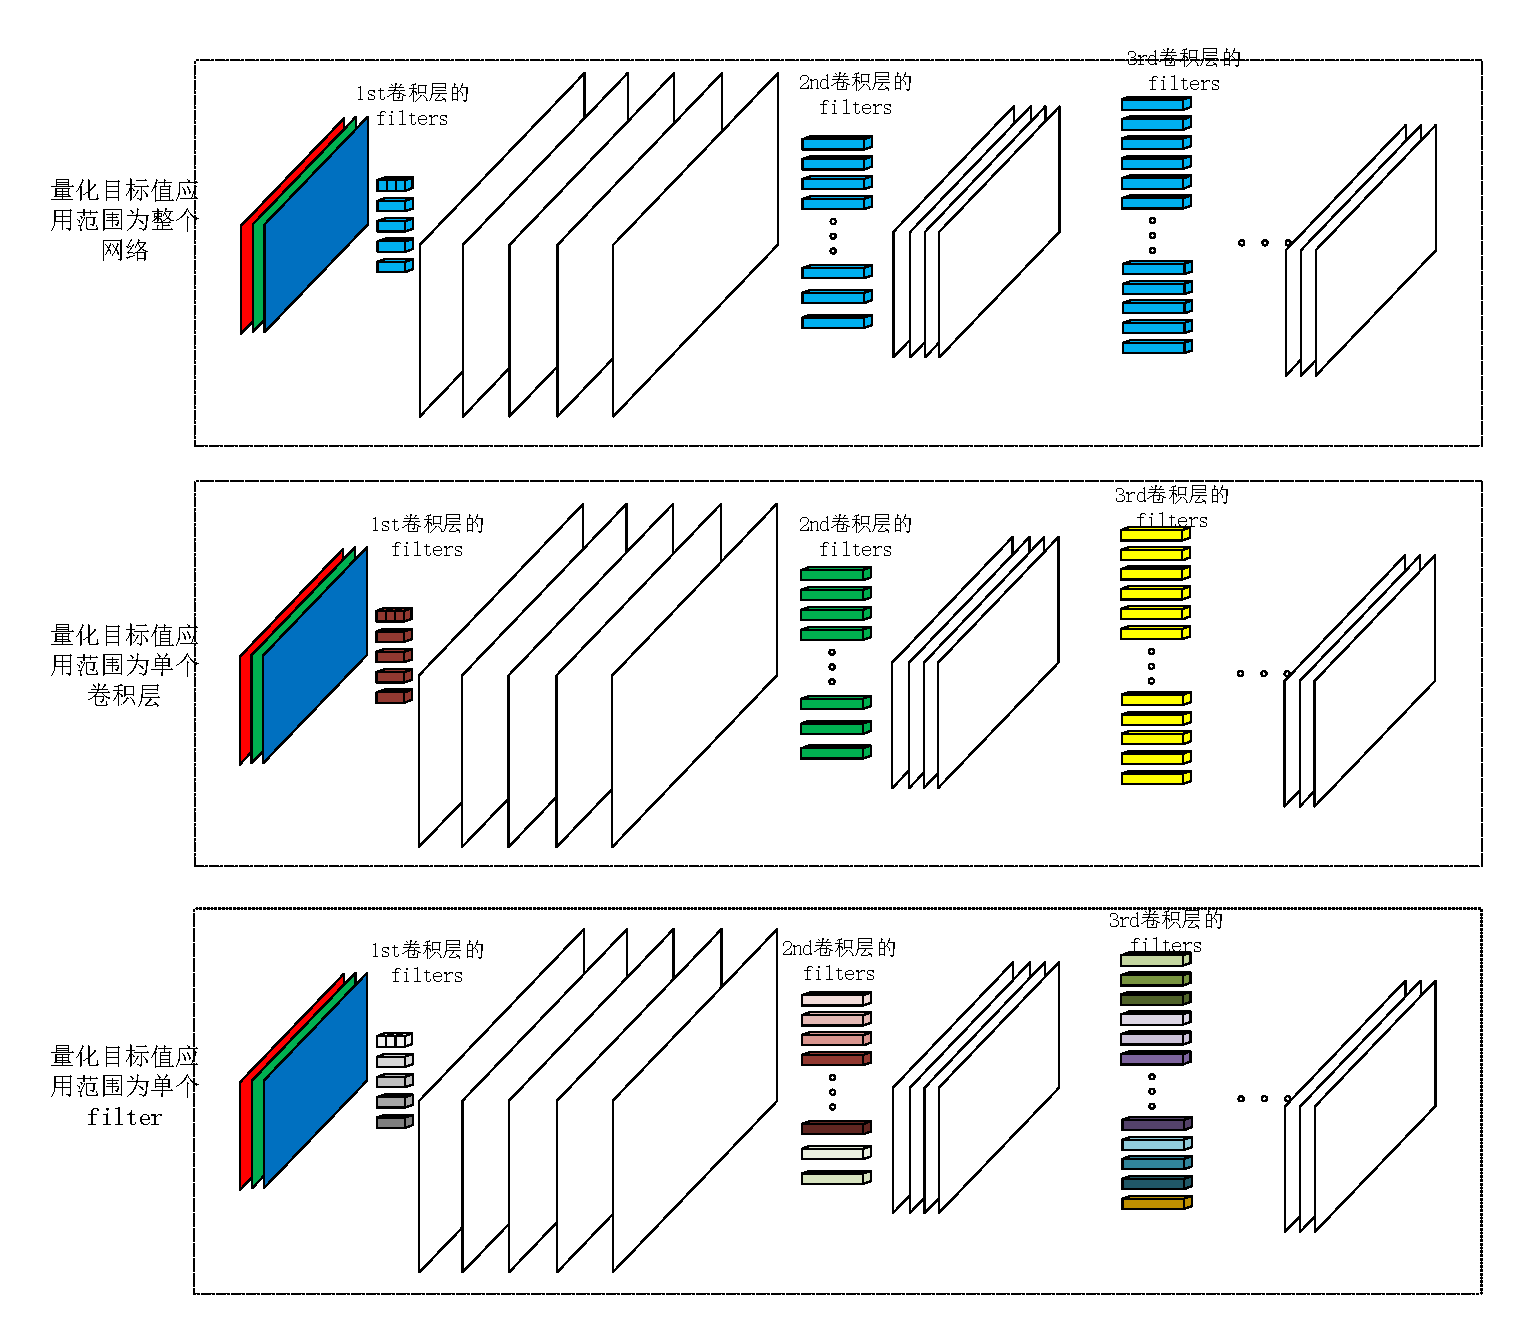
\includegraphics[width=\textwidth]{set_range.pdf}
\caption{三种量化目标值集合的应用范围的对比}
\label{set_range}
\end{figure}

图 \ref{set_range}中展示了三种量化目标值集合$Set_{target}$的应用范围。图中从左向右看是卷积网络卷积的全过程。图中重叠在一起的长方形是卷积网络输入的特征图像(输出特征图像)。图中最左侧是三张红、绿、蓝色的图片,表示卷积网络第一个卷积层的输入特征图是彩色图片。因为本章关注的是CNN网络参数的量化,又为了保证网络的完整、可读性,所以图 \ref{set_range}中画出每一个卷积层之后的输出特征图,但是并没有标记颜色。

卷积层可以看作是由多个filters构成的,每个filtet都包含该层的一部分参数。图 \ref{set_range}中,长方体表示filters,所以图中每个卷积层都由若干排成一列的filters长方体组成,即CNN网络中所有的长方体对应该网络中所有的参数。图 \ref{set_range}对filters进行了着色,颜色相同的filters在量化时,量化操作的目标值集合是相同的。比如最上面一行可以看作是对\cite{ternary}的一个描述。图中最上面的卷积网络中所有filters颜色都标记为蓝色,这表明整个网络中所有参数的量化目标值集合是相同的,就像\cite{ternary}中,整个网络参数的量化目标值都是$Set_{target} = \{-1, 0, 1\}$。最上方的CNN网络中,量化目标值集合的应用范围是整个CNN网络。在中间的CNN网络中,各个卷积层层内filters着色相同,而不同层的filters颜色不同。所以中间CNN网络图中,量化目标值集合的应用范围是某个卷积层。在图 \ref{set_range}最下方的CNN网络中,整个网络中所有filters的颜色都互不相同,这表明,在该网络中,量化目标值集合的应用范围是某特定个filters。

\subsection{调整量化目标值应用范围的必要性}

现有的量化算法之所以能实现对CNN计算的加速,依赖的是量化目标值比较特殊。量化目标值通常是2的幂值形式。量化算法对对模型存储的压缩需要控制量化后参数取值范围变小,即量化目标值集合$Set_ {target}$中元素要尽可能的少。
现有的量化算法,部分如\cite{incremental}、\cite{extremely}已经可以对网络进行几乎无损的量化,不过这类量化算法的量化目标值集合$Set_ {target}$中元素是比较多的

\begin{eqnarray}
Set_ {target}=\{\dots, -2^{n_1}, -2^{n_2}, \dots, 0, \dots, 2^{n_3}, 2^{n_4}, \dots\}
\end{eqnarray}

\noindent 而类似\cite{binary}、\cite{binary1}、\cite{ternary}、\cite{xnornet}一类量化算法比\cite{incremental}、\cite{extremely}对CNN有更好的压缩效果,但还不能在保证CNN分类精度的前提下,将网络参数量化。原因在于,这些算法\cite{binary}、\cite{binary1}、\cite{ternary}、\cite{xnornet}的量化目标值集合$Set_ {target}={-1,0,1}$或者$\{-1, 1\}$,集合$Set_ {target}$过小。这类算法\cite{binary}、\cite{ternary}、\cite{xnornet}之所以会导致CNN的精度损失,是因为各个卷积层参数在被这些算法量化之后,参数空间过小,算法收敛能力较差。

为了保证CNN被量化之后,存储参数需要的比特位数不变,但各个卷积层的参数空间能更大、更复杂一些,本章提出的解决方案就是调整量化目标值的应用范围。



\begin{figure}
\centering
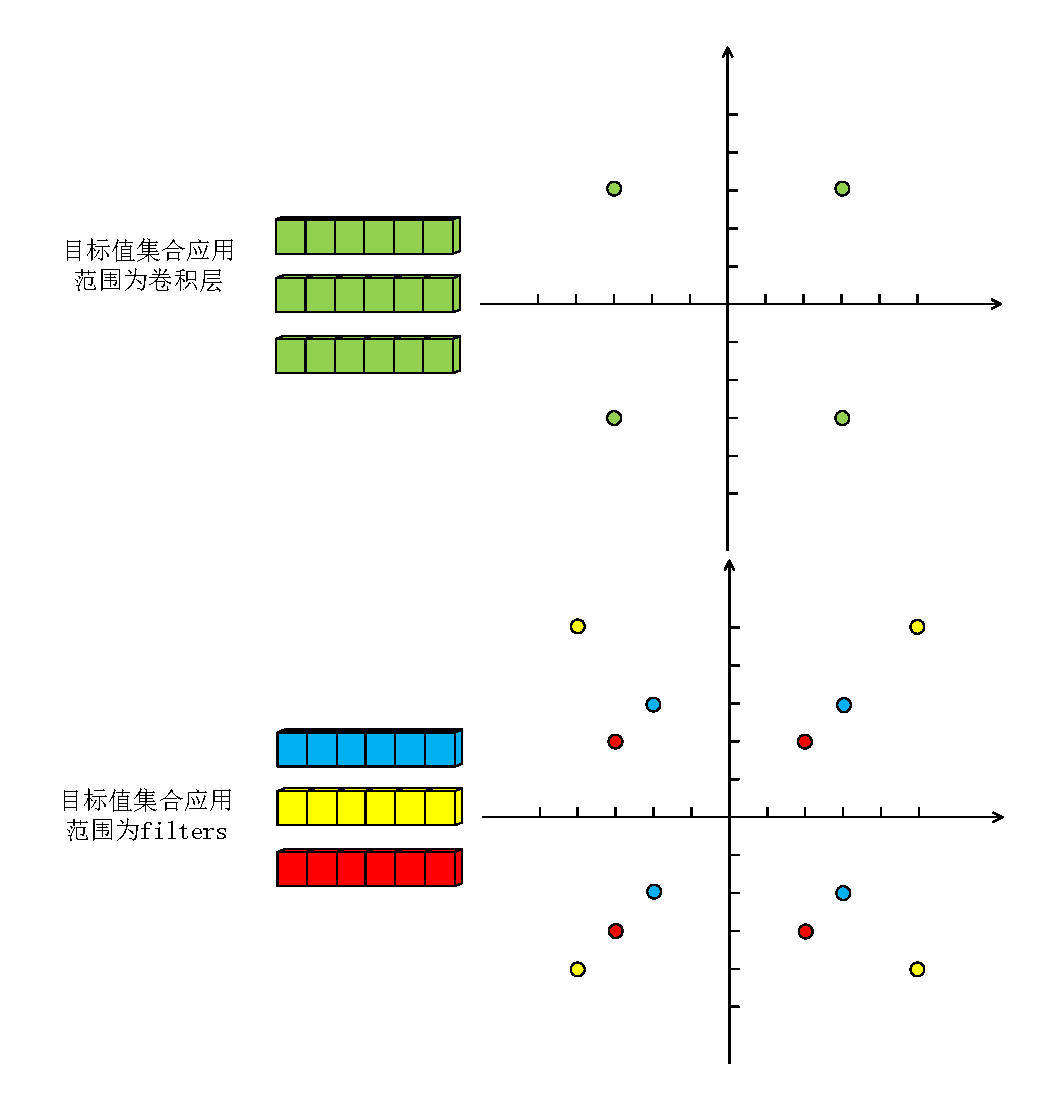
\includegraphics[scale=0.7]{param_range.pdf}
%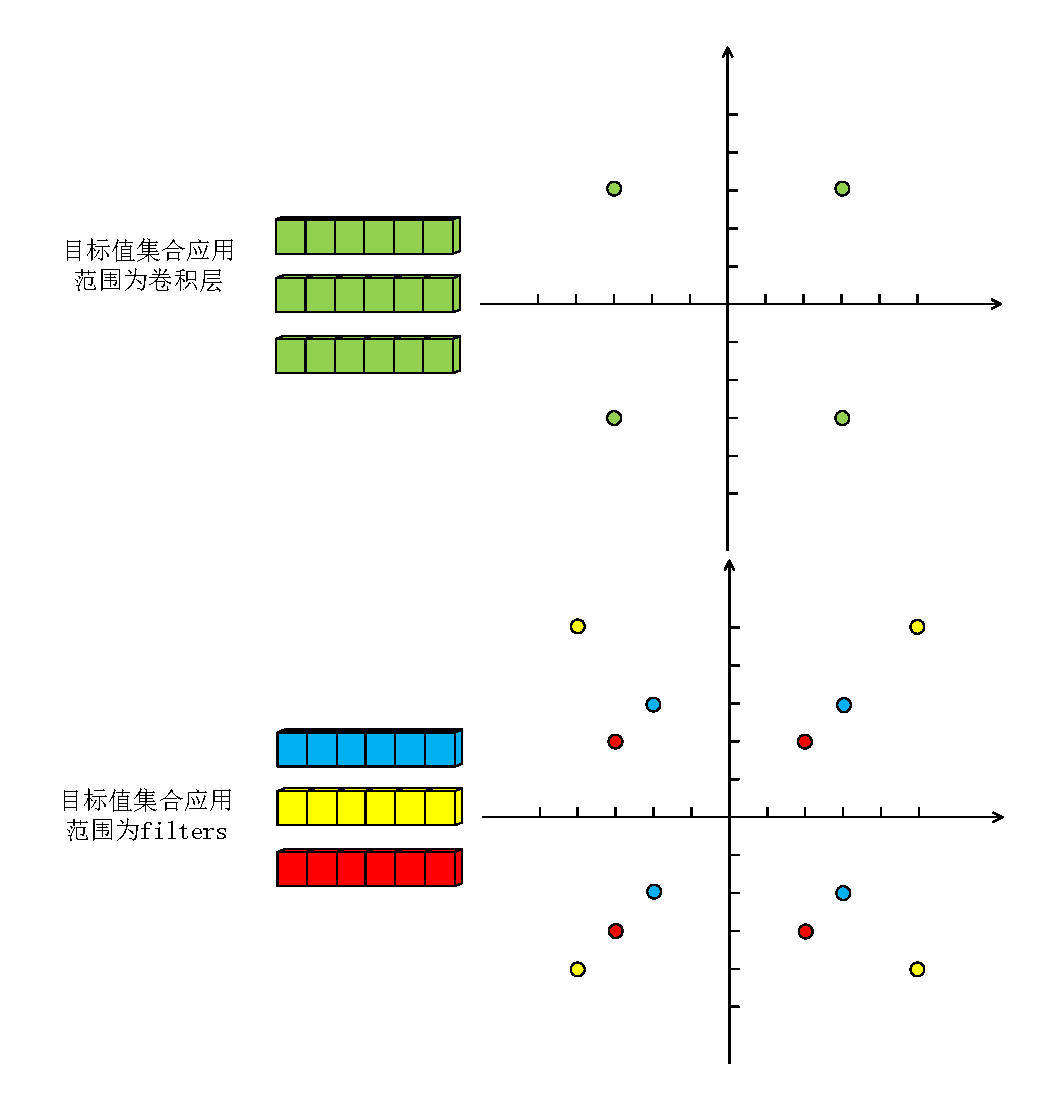
\includegraphics[width=\textwidth]{param_range.pdf}
\caption{两种目标值集合应用范围下,参数空间对比}
\label{param_range}
\end{figure}

%\noindent

在图 \ref{param_range}中,展示了两种不同的量化目标值集合应用范围。图中仅画了一个卷积层,简单说明改变应用范围的好处。图中长方体指的是filters,右侧二位坐标系里的点表示的参数空间。图中相同颜色的filters和坐标系中点,表示对应关系。图 \ref{param_range}中规定了量化后的参数存储只能占1比特,所以量化目标值集合$Set_ {target} = \{x_1, x_2\}$,即该集合只包含两个值。图 \ref{param_range}中上半部分描述的是\cite{binary}中的情形,$Set_ {target} = \{-1, 1\}$,量化目标值应用范围为整个网络。因为$Set_ {target} = \{-1, 1\}$,所以对应的参数空间坐标为

\begin{eqnarray}
\{(-1,-1), (-1,1), (1,-1), (1,1)\}
\end{eqnarray}

\noindent当量化目标值的应用范围为整个网络时,所有的filters对应的参数参数空间都是同样的四个点。图 \ref{param_range}中下半部分描述的是量化目标值集合应用范围为filters时的情形。因为应用范围为filters,所以每个filters都有各自对应的目标值集合,本章用$Set_ {target,i} = \{x_{i,1}, x_{i,2}\}$表示第i个filters对应的集合,其中i表示第i个filters,$x_{i,j}$表示第i个filter的第j个量化目标值(图中j取值范围为1、2),且$x_{i,j}$数值为2的幂值形式。$Set_ {target,i} = \{x_{i,1}, x_{i,2}\}$对应的参数空间为

\begin{eqnarray}
\{(x_{i,1}, x_{i,1}), (x_{i,1}, x_{i,2}), (x_{i,2}, x_{i,1}), (x_{i,2}, x_{i,2})\}
\end{eqnarray}

\noindent 因为每个filter都有各自的目标值集合$Set_ {target,i} = \{x_{i,1}, x_{i,2}\}$,所以图中下方的卷积层对应的参数空间比上方复杂得多。

通过图 \ref{param_range}可以发现,在参数用相同的1比特表示的情况下,当目标值集合的应用范围从整个网络(或者卷积层)调整为filters时,CNN网络对应的参数空间更复杂。
而且调整目标值应用范围之后,基于特定的硬件,计算复杂度上也几乎不会上升。以图 \ref{param_range}中情况为例。原\cite{binary}中目标值为-1、1,卷积中乘法运算可以转化为对浮点数的符号位的位运算,该位运算需要消耗一个指令周期。调整集合应用范围之后,因为目标值为$\pm 2^n$形式,所以卷积核进行卷积时,浮点数乘法被转换为符号位与位移运算。在具体硬件实现时,可以通过可以设置两个缓冲器,分别记录是否进行符号位运算以及记录位移运算位移的位数,在一个指令周期中,完成上述两个位运算。

\section{量化目标值集合计算}

本章尝试调整了量化目标值集合的应用范围,目的是希望该集合和它应用范围内的参数尽可能契合。假设将全网络的参数分为n个应用范围,这n个范围内的参数用集合$W_i = \{x_1, x_2, \dots, x_l\}$表示,其中$W_i$表示第i个应用范围内的参数集合,x表示单个参数。针对这个n个应用范围,将生成n个不同的量化目标值集合$Set_ {target,i} = \{\dots, 2^{n_{i,1}}, 2^{n_{i,2}}, 2^{n_{i,3}}, \dots\}$,其中i的取值范围为$\{1, 2, \dots, n\}$, $n_{i,1}$为整数,且$n_{i,j}<n_{i,(j+1)}$。

根据第一段中的定义可以发现,量化算法的目标是最终将$W_i$内的元素,用$Set_ {target,i}$内的元素替换。那么很显然,为了保证量化后模型精度,本文认为参数替换时的误差尽可能小。为了定义这个误差,本章首先定义一些函数。为了优化计算速度,$Set_ {target,i}$内的元素都是$2^n$的形式。首先定义了量化函数quan(x):

%\begin{eqnarray}
%\text{$\forall x \in W_i:$}
%\text{if}
 %\text{$2^n \in Set_{target,i},$}
 %\text{$\forall n_{i,j},|x-2^n| \leq |x-2^{n_{i,j}}|$}
%\text{$then:$}
%quan(x) = 2^{n},

%\label{3quantization}

%\end{eqnarray}


\begin{eqnarray}
\hat x = quan(x) = \gamma,
\gamma \in Set_{target,i},
\forall y \in Quan_{set}, |\gamma - x|<= |y - x|,
\label{quan}
\end{eqnarray}

根据量化函数quan(x)的定义,将量化目标值集合的确定过程看作一个优化过程:

\begin{eqnarray}
min \sum_{x \in W_i}|x-quan(x)|^2
\end{eqnarray}

为了便于求解,适当对上述优化做了放缩。首先定义求绝对值的函数abs(x)和求均值的函数$mean(W_i)$:

\begin{eqnarray}
abs(x) = \begin{cases}
		-1*x,& \text{如果} x < 0; \\
		x,& \text{如果} x \geq 0.
		\end{cases}
\end{eqnarray}

\begin{eqnarray}
mean(W_i) = \frac{n}{1}\sum_{i=1,2,\dots,n}abs(x_i) ,( \forall x_i, x_i \in W_i );
\end{eqnarray}

那么对某一应用范围内的参数$W_i = \{x_{i,1}, x_{i,1}, \dots, x_{i,n}\}$,量化目标值集合可以定义为$Set_ {target,i} = \{-t, t\}$,其中t的取值为:

\begin{eqnarray}
t = quan(mean(abs(W_i)))
\label{new.quan}
\end{eqnarray}。



\section{二值化的量化算法及其改进}

\subsection{以CNN网络为应用范围的原二值化算法思路}

在\cite{binary}中,作者尝试将CNN网络中的参数量化为$Set_ {target,i} = \{-1,1\}$。在该算法中,作者定义了参数量化公式:

\begin{eqnarray}
quan(x) = sign(x) = \begin{cases}
		1,& \text{如果} x < 0; \\
		-1,& \text{如果} x \geq 0.
		\end{cases}
\end{eqnarray}

在\cite{binary}中,作者根据如下流程来训练二值化的CNN网络:

\begin{algorithm}[htb]
  \caption{\cite{binary}中的量化算法}
  \label{41training}
  \begin{algorithmic}[1]
    \REQUIRE
      训练集:X, 量化目标值集合$Set_ {target,i} = \{-1,1\}$,最大训练周期数N: $epoch_{max}$,
      量化函数:quan(x); 学习率:$\eta$;
      \\
    \ENSURE 模型第L层的参数为:${W_l, 1\leq l\leq L}$;
    \STATE 初始化模型参数: ${W_l}$, ${1\leq l\leq L}$, $\eta$, $epoch_{max}$。
    \STATE 如果模型没有收敛且$epoch<epoch_{max}$:
    \STATE \qquad 对于 l = 1, 2, $\ldots$, L:
    \STATE \qquad \qquad 保存网络各层参数 $tmp\_W_l=W_l$
    \STATE \qquad \qquad $\hat{W_l}=quan(W_l)$
    \STATE \qquad 根据训练集X,CNN网络进行前向计算(forward)

    \STATE \qquad 根据训练集X,反向传播,计算网络参数$W_l$的梯度$grad_l$;
    \STATE \qquad 对于 l = 1, 2, $\ldots$, L:
    \STATE \qquad \qquad 恢复网络各层参数 $W_l = tmp\_W_l$
    \STATE \qquad \qquad 根据$grad_l$更新参数$W_l$: $W_l = W_l+ \eta*grad_l$
    \STATE Return 返回训练完的量化模型;
  \end{algorithmic}
\end{algorithm}

如算法.\ref{41training}中所述,在\cite{binary}算法中,作者在前向(forward)计算时,会首先根据量化算法quan(x)将所有的参数$W_l$,量化为$Set_ {target,i} = \{-1,1\}$中的某个值。此时,量化完的网络是一个由-1,1组成的二值化网络,参数为$\hat{W_l}$。当然,最开始这个由1,-1作为参数的网络是没收敛的,在分类测试集上精度不高。接着,根据正向计算、梯度的反向传播,求出二值化网络中各个参数的梯度$grad_l$。此时\cite{binary}中并没有直接根据梯度更新二值化的参数,而是恢复了网络的原参数$W_l$(未二值化,浮点数参数),然后利用$grad_l$更新了参数$W_l$。以上操作将持续进行,直至网络被训练到收敛。

\subsection{以filters为应用范围的二值化算法思路}

不同于现有的很多工作,尝试改进\cite{binary}的量化策略。本章的改进思路在于调整量化目标值集合的应用范围。原\cite{binary}中,整个网络参数都被量化为$Set_ {target} = \{-1,1\}$,即整个CNN网络中,所有filters中的参数都将被量化为-1,1。调整量化目标值应用范围之后,整个网络中各层、每层内不同的filters都将有各自的量化目标值集合$Set_ {target,l,j} = \{-t_{l,j},1-{l,j}\}$,其中l指的是该卷积核对应CNN网络第几个卷积网络,j对应第l个网络的第j个filter。

根据公式 \ref{new.quan},可以求出第l层,第j个filter的量化目标值集合$Set_ {target,l,j}$为:

\begin{eqnarray}
Set_ {target,l,j} = quan(mean(abs(W_{l,j})))
\label{filter.quan}
\end{eqnarray}

在公式 \ref{filter.quan}中,$W_{l,j}$指的是,第l层第j个filter中的参数。改进后的算法流程可以表示为:

\begin{algorithm}[htb]
  \caption{基于filters确定量化目标值的量化算法}
  \label{2training}
  \begin{algorithmic}[1]
    \REQUIRE
      训练集:X, 第l个卷积层的第j个filter参数:$SW_{l,j}$,其中l的取值范围为$L = \{1,2,3,\dots,l_max\}$,j的取值范围为$J = \{1,2,3,\dots,j_{l,max}\}$;最大训练周期数N: $epoch_{max}$,
      量化函数:quan(x); 学习率:$\eta$;
      \\
    \ENSURE 模型第L层的参数为:${W_l, 1\leq l\leq L}$;
    \STATE 初始化模型参数: ${W_l}$, ${1\leq l\leq L}$, $\eta$, $epoch_{max}$。
    \STATE 如果模型没有收敛且$epoch<epoch_{max}$:

    \STATE \qquad 对于 l = 0, 1, $\ldots$, L-1:
    \STATE \qquad \qquad 对于 j = 0, 1, $\ldots$, J-1:
    \STATE \qquad \qquad \qquad 计算${filter_l,j}$的量化目标值集合$Set_ {target,l,j}$;

    \STATE \qquad 对于 l = 0, 1, $\ldots$, L-1:
    \STATE \qquad \qquad 对于 j = 0, 1, $\ldots$, J-1:
    \STATE \qquad \qquad \qquad 保存网络各层参数 $tmp\_W_{l,j}=W_{l,j}$
    \STATE \qquad \qquad \qquad 根据量化目标值集合$Set_ {target,l,j}$,求$\hat{W_{l,j}}=quan(W_{l,j})$
    \STATE \qquad 根据训练集X,CNN网络进行前向计算(forward)

    \STATE \qquad 根据训练集X,反向传播,计算网络参数$W_{l,j}$的梯度$grad_{l,j}$;
    \STATE \qquad 对于 l = 0, 1, $\ldots$, L-1:
    \STATE \qquad \qquad 对于 j = 0, 1, $\ldots$, J-1:
    \STATE \qquad \qquad \qquad 恢复网络各层参数 $W_{l,j} = tmp\_W_{l,j}l$
    \STATE \qquad \qquad \qquad 根据$grad_l$更新参数$W_{l,j}$: $W_{l,j} = W_{l,j}+ \eta*grad_{l,j}$
    \STATE Return 返回训练完的量化模型;
  \end{algorithmic}
\end{algorithm}



\section{实验及结果分析}

\subsection{实验设置}
对比实验数据集,本章选了Fashion-MNIST、SVHN、CIFAR10数据集,对比网络采用了AlexNet和VGG19网络。实验的实现细节如上一个段落中算法流程所述。

\subsection{实验结果}
基于Fashion-MNIST数据集,本章对两个网络:AlexNet行了二值化操作。进行二值化操作时,本章选择了\cite{binary}算法;之后基于调整化目标值范围的思路,对CNN网络各个filters计算相应的二值化目标值集合,之后进行与\cite{binary}同样的二值化训练过程。基于相同的二值化策略\cite{binary},我们对比了原二值化目标集合以及基于filters优化后量化目标值的量化效果。

基于SVHN数据集,本章对两个网络:AlexNet和VGG19进行了二值化操作。进行二值化操作时,本章选择了\cite{binary}算法;之后基于调整化目标值范围的思路,对CNN网络各个filters计算相应的二值化目标值集合,之后进行与\cite{binary}同样的二值化训练过程。基于相同的二值化策略\cite{binary},我们对比了原二值化目标集合以及基于filters优化后量化目标值集合的量化效果。

基于CIFAR10数据集,本章对两个网络:AlexNet和VGG19进行了二值化操作。进行二值化操作时,本章选择了\cite{binary}算法;之后基于调整化目标值范围的思路,对CNN网络各个filters计算相应的二值化目标值集合,之后进行与\cite{binary}同样的二值化训练过程。基于相同的二值化策略\cite{binary},我们对比了原二值化目标集合以及基于filters优化后量化目标值集合的量化效果。

由于二值化网络的训练是比较难以收敛的,因此实验中设定了最高训练周期数。

\begin{table}[!htbp]
\caption{基于Fashion-MNIST数据集,不同量化目标值应用范围,AlexNet量化结果的对比}
\begin{tabular}{|c|c|c|}
\hline
- & 以网络为单位\cite{binary}$Accuracy(\%)$  & 以filters为单位$Accuracy(\%)$  \\ \hline
\multicolumn{3}{|c|}{AlexNet} \\ \hline
baseline & 99.60 & 99.60  \\ \hline
$quan$ & 99.32 & 99.71 \\
\hline
\hline
\end{tabular}
\label{quan_range1}
\end{table}


\begin{table}[!htbp]
\caption{基于SVHN数据集,不同量化目标值应用范围,AlexNet和VGGNet量化结果的对比}
\begin{tabular}{|c|c|c|}
\hline
- & 以网络为单位\cite{binary}$Accuracy(\%)$  & 以filters为单位$Accuracy(\%)$  \\ \hline
\multicolumn{3}{|c|}{AlexNet} \\ \hline
baseline & 92.74 & 92.74  \\ \hline
$quan$ & 91.10 & 92.44 \\
\hline
\hline
\multicolumn{3}{|c|}{VGGNet} \\ \hline
baseline & 95.77 & 95.77  \\ \hline
$quan$ & 94.93 & 96.10 \\ \hline
\end{tabular}
\label{quan_range2}
\end{table}


\begin{table}[!htbp]
\caption{基于CIFAR10数据集,不同量化目标值应用范围,AlexNet和VGGNet量化结果的对比}
\begin{tabular}{|c|c|c|}
\hline
- & 以网络为单位\cite{binary}$Accuracy(\%)$  & 以filters为单位$Accuracy(\%)$  \\ \hline
\multicolumn{3}{|c|}{AlexNet} \\ \hline
baseline & 85.01 & 85.01  \\ \hline
$quan$ & 81.95 & 83.73 \\
\hline
\hline
\multicolumn{3}{|c|}{VGGNet} \\ \hline
baseline & 94.12 & 94.12  \\ \hline
$quan$ & 92.62 & 93.78 \\ \hline
\end{tabular}
\label{quan_range3}
\end{table}


\subsection{实验结果分析}

在表 \ref{quan_range1}、表\ref{quan_range2}和表\ref{quan_range3}的对比实验中,二值化参数的思想和流程是相同的,不同的是,二值化操作的目标值集合。原\cite{binary}中,整个CNN网络中所有的参数都被量化到相同的目标值集合$Set_{target} = {-1,1}$中。而对比实验中调整了二值化目标值集合的应用范围,算法针对各个filters生成对应的量化集合$Set_ {target,l,j}$。表  \ref{quan_range}中,AlexNet指的是AlexNet模型相关预的对比数据;同理VGGNet指的是VGGNet模型相关的对比。这里$VGGNet$指的是$VGG16$网络结构。表格中的baseline,指的是训练得到的全精度(21位浮点数)参数的AlexNet或者VGGNet,在测试集上取得的测试精度。表格中,$quan$指的是,同样的网络,被量化之后在测试集上的分类精度。

从表 \ref{quan_range1}中可以看出,在Fashion-MNIST数据集上,AlexNet在全精度下的测试准确率为99.60%;而利用\cite{binary}中二值化的方法,量化之后的网络精度为99.32%;而根据各个filters生成相应的量化目标值,得到的量化网络精度为99.71%,精度上高于\cite{binary}中的二值化网络。

从表 \ref{quan_range2}中可以看出,在SVHN数据集上,AlexNet在全精度下的测试准确率为92.74%;而利用\cite{binary}中二值化的方法,量化之后的网络精度为91.10%;而根据各个filters生成相应的量化目标值,得到的量化网络精度为92.44%,虽然二值化后网络精度下降,但是基于filters生成目标值之后的二值化网络精度上显著高于原\cite{binary}中的二值化网络。在VGG19网络上,全精度下的测试准确率为95.77%;而利用\cite{binary}中二值化的方法,量化之后的网络精度为94.93%;而根据各个filters生成相应的量化目标值,得到的量化网络精度为96.71%,基于filters调整量化目标值不仅使得二值化后网络精度高于\cite{binary}中的二值化网络,甚至分类精度优于全精度网络。

从表 \ref{quan_range3}中可以看出,在CIFR10数据集上,AlexNet在全精度下的测试准确率为85.01%;而利用\cite{binary}中二值化的方法,量化之后的网络精度为81.95%;而根据各个filters生成相应的量化目标值,得到的量化网络精度为83.73%,精度上显著高于\cite{binary}中的二值化网络。在VGG19网络上,改变量化目标值集合应用范围也促进了二值化之后网络的分类精度。

综上所述,调整量化目标值集合的应用范围,针对不同的filters生成相应的量化目标值集合,既不会增加CNN模型的存储,还可以提升二值化算法的精度。

\section{本章小结}

近年来的很多工作都在试图对网络进行二值化,早期的\cite{binary}、\cite{binary1},到最近的\cite{extremely}、\cite{18bianry}。近年来的工作\cite{extremely}、\cite{18bianry}、\cite{cvprq71}尝试通过添加一个scale操作,来增加二值化网络的精度。但还几乎没有工作注意到通过对量化目标值集合的调整,生成对应的量化目标值集合,从而优化量化算法的得到的深度学习模型分类精度。我们的工作证明了针对filters生成相应的量化目标值集,能增强二值化网络的精度。调整量化目标值的应用范围,是能使量化算法精度提升的可行的方法。


%%%%%%

%%%%%%

\chapter{基于增量式少量预训练的剪枝算法(IPLT)}

\section{引言}

深度学习优化算法中,剪枝算法是一个大的类别。早期剪枝算法更重视对参数的剪枝。早期剪枝算法\cite{90prune}, \cite{92prune}主要集中在对卷积核参数的剪枝上,剪枝能够让卷积核稀疏化可以视为对模型的一种正则化,防止模型过拟合。2012年开始,深度学习模型大热,伴随着计算机算力的提升,人们设计出来的CNN模型越来越复杂,降低模型的存储占用空间和计算复杂读度成为了很多研究者的研究重心。伴随着这一背景,剪枝算法再次进入了人们的视野。不过不同于之前的剪枝工作,12年之后的剪枝算法目标是修建掉尽可能多的参数。这一时期的剪枝算法涌现了很多优秀的工作,如\cite{11},\cite{12}。在现有的普通的软件、硬件框架下,并不支持直接对稀疏卷积核的进行运算。参考稀疏矩阵的乘法运算的实现过程,可以发现这种稀疏化虽然可以压缩CNN网络模型存储,但是在实际稀疏CNN模型的运算需要依赖特定的库函数,虽然模型压缩效果不错,但加速效果并不能让人满意。

因为参数剪枝依赖特定库,加速效果并不好,16年之后,研究者\cite{17},\cite{13}开始尝试研究能基于现有深度学习框架直接运用的剪枝模型——对通道(channels)或者说filters的剪枝。本文将在下一部分中详细说明filters剪枝的细节原理。对filters的剪枝直接修改了CNN网络卷积层的尺寸,而没有稀疏化卷积核 ,所以并不需要特殊的库,现有深度学习框架就可以运行剪枝后的模型。

\begin{figure}
\centering
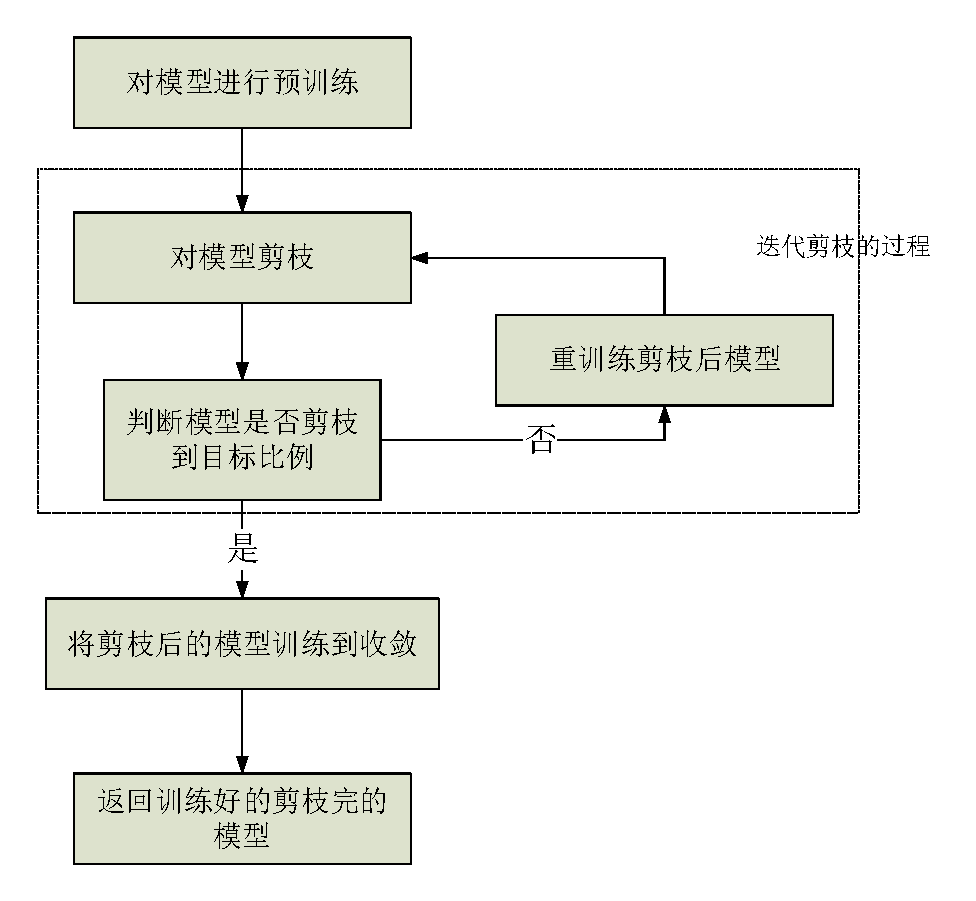
\includegraphics[width=\textwidth]{pruning_liucheng.pdf}
\caption{CNN网络进行剪枝的一般性流程}
\label{pruning_liucheng}
\end{figure}

不论是对filters的剪枝还是对参数的剪枝,在流程上都可以被总结为如图 \ref{pruning_liucheng}大致的一个过程。现有的剪枝算法都很依赖.\ref{pruning_liucheng}中最上方标明的预训练模型的阶段。基于对特定模型预训练的过程,剪枝算法之后将根据某种标准或者算法剪去模型的参数或者filters。一般现有的剪枝算法,很难一次性将模型修剪到一个比较高的剪枝比例。比如,假设剪枝算法的目标是将CNN网络中90\%的参数或者filters剪去,那么现有的剪枝算法是几乎不能一次剪枝操作剪掉这么多参数或filters。这是因为,每次剪枝操作如果剪去的filters过多,那么模型的精度将会受到极大的影响。所以现有的剪枝算法都有一个如图 \ref{pruning_liucheng}中虚线方框所示的,迭代剪枝的过程。

迭代剪枝的思想很简单:1.在执行剪枝算法的时候,每次剪枝操作都只剪去很少一部分的filters或参数;2.继续训练剩下的模型,让模型恢复精度;3.执行下一次剪枝操作,少量剪枝。如此循环,直到模型被修剪到预限设定的大小。

现有剪枝算法的预训练阶段往往会将模型训练到收敛,这一过程通常有200~300epochs。现有的剪枝算法有大量预训练,却不能一次性有效地将模型剪枝到目标大小。本文认为,需要思考一个问题:这样过量的预训练是否真的有必要。1.既然对模型进行大量的预训练,现有剪枝算法也不能一步将模型剪枝到位;2.迭代剪枝,每步剪枝少量参数或filters往往能取得比较好的剪枝效果。结合以上两个点,本文认为,如果每次剪枝都只是剪去少量参数,很可能完全没必要进行大量的预训练,只需要少量的预训练就有可能实现比较好的剪枝效果。

针对这个想法,本章中提出了一种基于少量预训练的、增量式剪枝思想(incremental pruning thought based less training,简称IPLT)。这个思想大致思想就是基于少量预训练就开始剪枝,每次剪少量的参数。该工作主要有两点贡献:1.新颖性:该工作是现有剪枝算法中第一个对剪枝算法必要的预训练数量进行思考的工作;2.普适性:该思想几乎可以用来改进现有的所有剪枝算法;3.优化了训练模型的计算代价:IPLT思想可以优化了预训练阶段的计算消耗。现有剪枝算法关注点都在剪枝后的模型能否实现足够多的压缩、计算优化;还没有工作关注到剪出一个模型的这个过程中计算量消耗的优化。假设一共对一个模型预训练300epochs,现有剪枝算法在这300epochs中都是训练一个完整的模型,之后才开始迭代剪枝。在IPLT的思想中,基于少量预训练之后就开始对模型及进行剪枝,一般只在前3、40epochs之后就已经将模型剪到目标修剪比例。之后40~300epochs中,基于IPLT思想的剪枝算法中的训练的都是修剪完毕的模型,这个模型因为已经被修剪,不管是前向计算还是反向传播求梯度是,计算量都远小于未剪枝的模型。

本章,第二部分将介绍filters剪枝的原理。之后的章节将介绍两个现有的剪枝算法\cite{17}, \cite{27},并用IPLT思想去改造这两个剪枝算法,进行了对比试验。




\section{filters剪枝算法}

\subsection{filters剪枝原理}

图 \ref{filters_pruning}详细展示了filters剪枝的原理。图中,我们对第i层的filters进行了剪枝,我们选择了第二和第四个filters进行修剪。我们会发现第i个卷积层输出的特征图中,第二、四张特征图因为filters被剪去,而同样被“剪去”。这时候,第$(i+1)$层的输入特征图少了两张,因此第$(i+1)$层所有filters中原来用来卷积第二、四特征图的参数因随之剪去。所以我们会发现图中,蓝色表示的第$(i+1)$层filters中有一些白色部分,就表示的这些被剪去的参数。

\begin{figure}
\centering
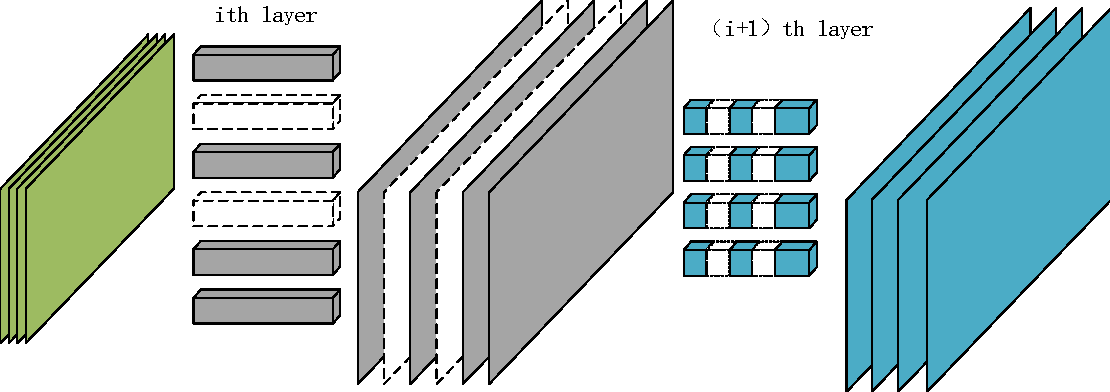
\includegraphics[width=\textwidth]{filters_pruning.pdf}
\caption{CNN网络filters剪枝的原理示意图}
\label{filters_pruning}
\end{figure}

因为剪枝算法是围绕卷积层进行的,所以图中画层都是指卷积层。图中重叠在一起的长方形表示的是各层的输入特征图或者输出特征图。本章用$Map_{l,in}$表示第l层卷积层的输入特征图,$Map_{l,out}$表示第i层的输出特征图。那么显然能够得到

\begin{eqnarray}
Map_{(l+1),in} == Map_{l,out}
\label{2fin.fout}
\end{eqnarray}

即第$(i+1)$层的输入特征图,实质上是第$i$层的输出特征图。

图中的长方体是filters,图中每一列filters表示同一个卷积层中的所有filters。图 \ref{filters_pruning}中的诸多filters,即相当于图 \ref{convolution}中第一个卷积层中三个诸多正方形叠成的长方体。结合图 \ref{convolution}可以看出,每个filter会将输入通道中的所有图像,卷积成一张特征图,所以某层如果有10个filters,那么该卷积层的输出特征图数量为10 ,下一层的输入特征图数量为10。所以每个filter中参数数量是由filter所在卷积层输入特征图数量决定的:本章用$F_{l,i}$表示第$l$个卷积层中第$i$个filter的参数数量。假设每个filetr中卷积都是$3*3$大小的,第$l$层共有$in_{l}$个特征图,那么第$l$层中第$i$中个filter中参数个数满足

\begin{eqnarray}
F_{l,i} = in_{l}*3*3
\end{eqnarray}

假设第$l$层共有$out_{l}$个特征图,本章用$F_l$表示第$l$层中共有的参数个数,那么$F_l$满足

\begin{eqnarray}
F_{l,i} = out_{l}*in_{l}*3*3
\end{eqnarray}

通过上面的描述可以看出,任一卷积层中filters数量和该层的输出特征图数量是相同的。当对某个卷积层的filters进行剪枝操作之后,该层的输出特征图$Map_{l,out}$数量$out_{l}$会跟着减少。在图 \ref{filters_pruning}中展示了相邻两个卷积层。剪去$ith$层的第2和第4个filters之后(图中白色虚线的filters),$ith$层的输出特征图中第2和第4张也被标记为白色、虚线,这表明因为对应filters被剪去,这两张输出特征图也不存在了。同时根据图像可以看出,当对第i层进行filters剪枝时,第$(i+1)th$层会做出相应改变。这是因为根据Forumla.\ref{2fin.fout},第$l$层输出的特征图即为下一层的输入特征图,第第$l$层filters被剪去(输出特征图被剪去),下一层的输入特征图变少了。图 \ref{filters_pruning}中第$(l+1)$层的filters中,用来卷积原第2和第4幅输入特征图的卷积已经没有用处了,也应当跟着被剪去。


\subsection{经典的剪枝算法}

\cite{17}中的剪枝算法,根据filters的范数值来度量filters的重要性,是filters剪枝算法领域中的经典算法。

\cite{17}中的算法流程大致如下面算法.\ref{17pruning}:

\begin{algorithm}[htb]
  \caption{\cite{17}中剪枝算法流程}
  \label{17pruning}
  \begin{algorithmic}[1]
    \REQUIRE
      训练集:X, 训练最大周期数: $epoch_{max}$,
      目标剪枝比例:tr,
      模型已剪枝比例:r=0
      每次剪枝操作的剪枝比例:$new_r$
      网络参数: $\mathcal{W} = \left\{\mathcal{W}_i , 1\leq i \leq L \right\}$,
      一个CNN模型, ${W_l,1\leq l\leq L}$;\\
    \ENSURE 模型第L层的参数为:${\hat{W_l}, 1\leq l\leq L}$;
    \STATE 初始化模型参数: ${W_l}$, ${1\leq l\leq L}$ ;
    \STATE 如果模型没有收敛且$epoch<epoch_{max}$:
    \STATE \qquad 训练 CNN 模型;
    \STATE \qquad epoch = epoch+1
    \STATE 如果$r < tr$, 执行:
    \label{code:fram:add}
    \STATE \qquad 根据$l2$范数公式,计算整个网络filters$\mathcal{F}_{i,j}, 1\leq j \leq I_i$ 的重要性;
    \STATE \qquad 对整个网络的filters进行重要性排序(global模式);
    \STATE \qquad 执行剪枝操作,剪去$new_r$比例的的filters;
    \STATE \qquad r = r + $new_r$
    \STATE \qquad Retraining剩下的模型,直到收敛;
    \STATE Return 剪枝完,训练完的模型;
  \end{algorithmic}
\end{algorithm}

现有的剪枝算法往往依赖某种标准对filters进行一个重要性排序,然后根据重要性,优先将不那么重要的filters剪去。

剪枝操作前第一步是要计算filters的重要性。在\cite{17}中作者采用了$l1$和$l2$范数数值作为filters的重要性,本章中简称\cite{17}中的剪枝算法为经典剪枝算法。假设用$F_{l,i}$表示第$l$个卷积层的第$i$个filter,filter的参数尺寸为$in_l*3*3$($in_l$为第l个卷积层的输入特征图数量)。本章定义filters重要性度量函数为$Imp(x)$,x为某个filter。计算filters的$l1$范数公式为公式 \ref{l1}:

\begin{equation*}
Imp(F_{l,i})_1 =  \sum_{m=1}^{in_l}\sum_{n=1}^3\sum_{k=1}^3 |x_{m,n,k}|
\label{l1}
\end{equation*}

计算filters的$l2$范数公式为公式 \ref{l2}:

\begin{equation*}
Imp(F_{l,i})_2 =  \sqrt[2]{\sum_{m=1}^{in_l}\sum_{n=1}^3\sum_{k=1}^3 x_{m,n,k}^2}
\label{l2}
\end{equation*}

第二步是要对filters进行重要性排序。通常有两种模式:1.intra-layer模式:每层层内filters进行重要性比较,一般选择这种比较方式各层剪filters的比例是相同的;2.global模式:将整个网络各层filters放在一起比较,这种比较模式下,一般各层filters被剪去的比例是不同的。\cite{17}中选择的是global的比较模式。


\subsection{原Soft剪枝算法流程介绍}

不同于之前的剪枝算法,\cite{27}在执行剪枝操作时,实际上只是将被选中、要“剪去”的filters的参数设置为0,并且这部分被“剪去”的filters将继续被更新。作者将这种剪枝思想为算法称为“Soft Filter Pruning”,因此本文中这种算法简称为“Soft剪枝”。

\cite{27}中的算法流程大致如下面算法.\ref{27pruning}:

\begin{algorithm}[htb]
  \caption{\cite{27}中剪枝算法流程}
  \label{27pruning}
  \begin{algorithmic}[1]
    \REQUIRE
      训练集:X, 训练最大周期数: $epoch_{max}$,
      目标剪枝比例:tr,
      %模型已剪枝比例:r=0
      %每次剪枝操作的剪枝比例:$new_r$
      网络参数: $\mathcal{W} = \left\{\mathcal{W}_i , 1\leq i \leq L \right\}$,
      一个CNN模型, ${W_l,1\leq l\leq L}$;\\
    \ENSURE 模型第L层的参数为:${\hat{W_l}, 1\leq l\leq L}$;
    \STATE 初始化模型参数: ${W_l}$, ${1\leq l\leq L}$ ;
    \STATE 如果模型没有收敛且$epoch<epoch_{max}$:
    \STATE \qquad 训练 CNN 模型;
    \STATE \qquad epoch = epoch+1
    %\STATE 如果$r < tr$, 执行:

    \STATE \qquad 根据$l2$范数公式,计算整个网络filters$\mathcal{F}_{i,j}, 1\leq j \leq I_i$ 的重要性;
    \STATE \qquad 对整个网络的filters进行重要性排序(global模式);
    \STATE \qquad 执行剪枝操作,将$tr$比例的的filters中参数设置为0;

    \STATE \qquad Retraining整个模型;
    \STATE Return 剪枝完,训练完的模型;
  \end{algorithmic}
\end{algorithm}

\cite{27}是最近的工作,被发表在IJCAI2018上。这篇文章比较新颖,主要在于剪枝思路上并不是简单的直接剪去filters,而是soft剪法,每次剪枝操作并不将模型filters真实地剪去,而是将这部分filters置0,然后整个网络(包括置0的filters)一起继续训练,当模型训练完之后,一次性真实地剪去需要剪的filters。这种Soft剪枝的思想使得网络获得了更好的剪枝效果——在不影响模型精度的前提下,剪枝比例更高。本章中将这种剪枝算法简称为Soft剪枝。

\cite{27}首先需要设定一个超参:目标剪枝比例,tr。该剪枝执行Soft剪枝前也要计算filters的重要性。在\cite{27}中作者采用了$l2$范数数值作为filters的重要性。假设用$F_{l,i}$表示第$l$个卷积层的第$i$个filter,filter的参数尺寸为$in_l*3*3$($in_l$为第l个卷积层的输入特征图数量)。本章中定义filters重要性度量函数为$Imp(x)$,x为某个filter。计算filters的$l2$范数公式为公式 \ref{l2}:

\begin{equation*}
Imp(F_{l,i})_2 =  \sqrt[2]{\sum_{m=1}^{in_l}\sum_{n=1}^3\sum_{k=1}^3 x_{m,n,k}^2}
\label{l2}
\end{equation*}

第二步是要对filters进行重要性排序。\cite{27}中算法采用了global模式的filters重要性排序模式。假设该CNN网络中filters数量共为$num$个,那么每轮epoch将模型训练完之后,\cite{27}都会选出$tr*num$个filters,并将这些filters中的参数设置为0,然后进行下一轮epoch的训练。以上Soft剪枝的步骤将持续到模型收敛。

%##########################


\section{基于IPLT思想改进的剪枝算法}

本段落第一部分将首先介绍IPLT思想的详细细节。之后两个小节会介绍两个现有的剪枝策略\cite{17}和\cite{27},并用IPLT思想去改造这两个算法,完成对比实验。

\subsection{基于少量预训练的增量式剪枝思想(IPLT)}

本文提出了一种基于少量预训练的增量式剪枝思想(incremental pruning thought based less pre-training,简称IPLT)。IPLT思想其实并不复杂,简单说的话,就是跳过大量的预训练阶段,仅仅少量预训练之后就开始进行剪枝。因为预训练不多,所以模型还没有收敛,这时如果一次性对CNN的剪枝操作剪枝比例太高很容易影响剪枝后模型的性能,所以这里引入了增量式的思想。增量式思想本质就是少量多次。在图 \ref{pruning_contrast2}中展示了经过IPLT思想改进的剪枝算法和传统算法的对比图。

\begin{figure}
\centering
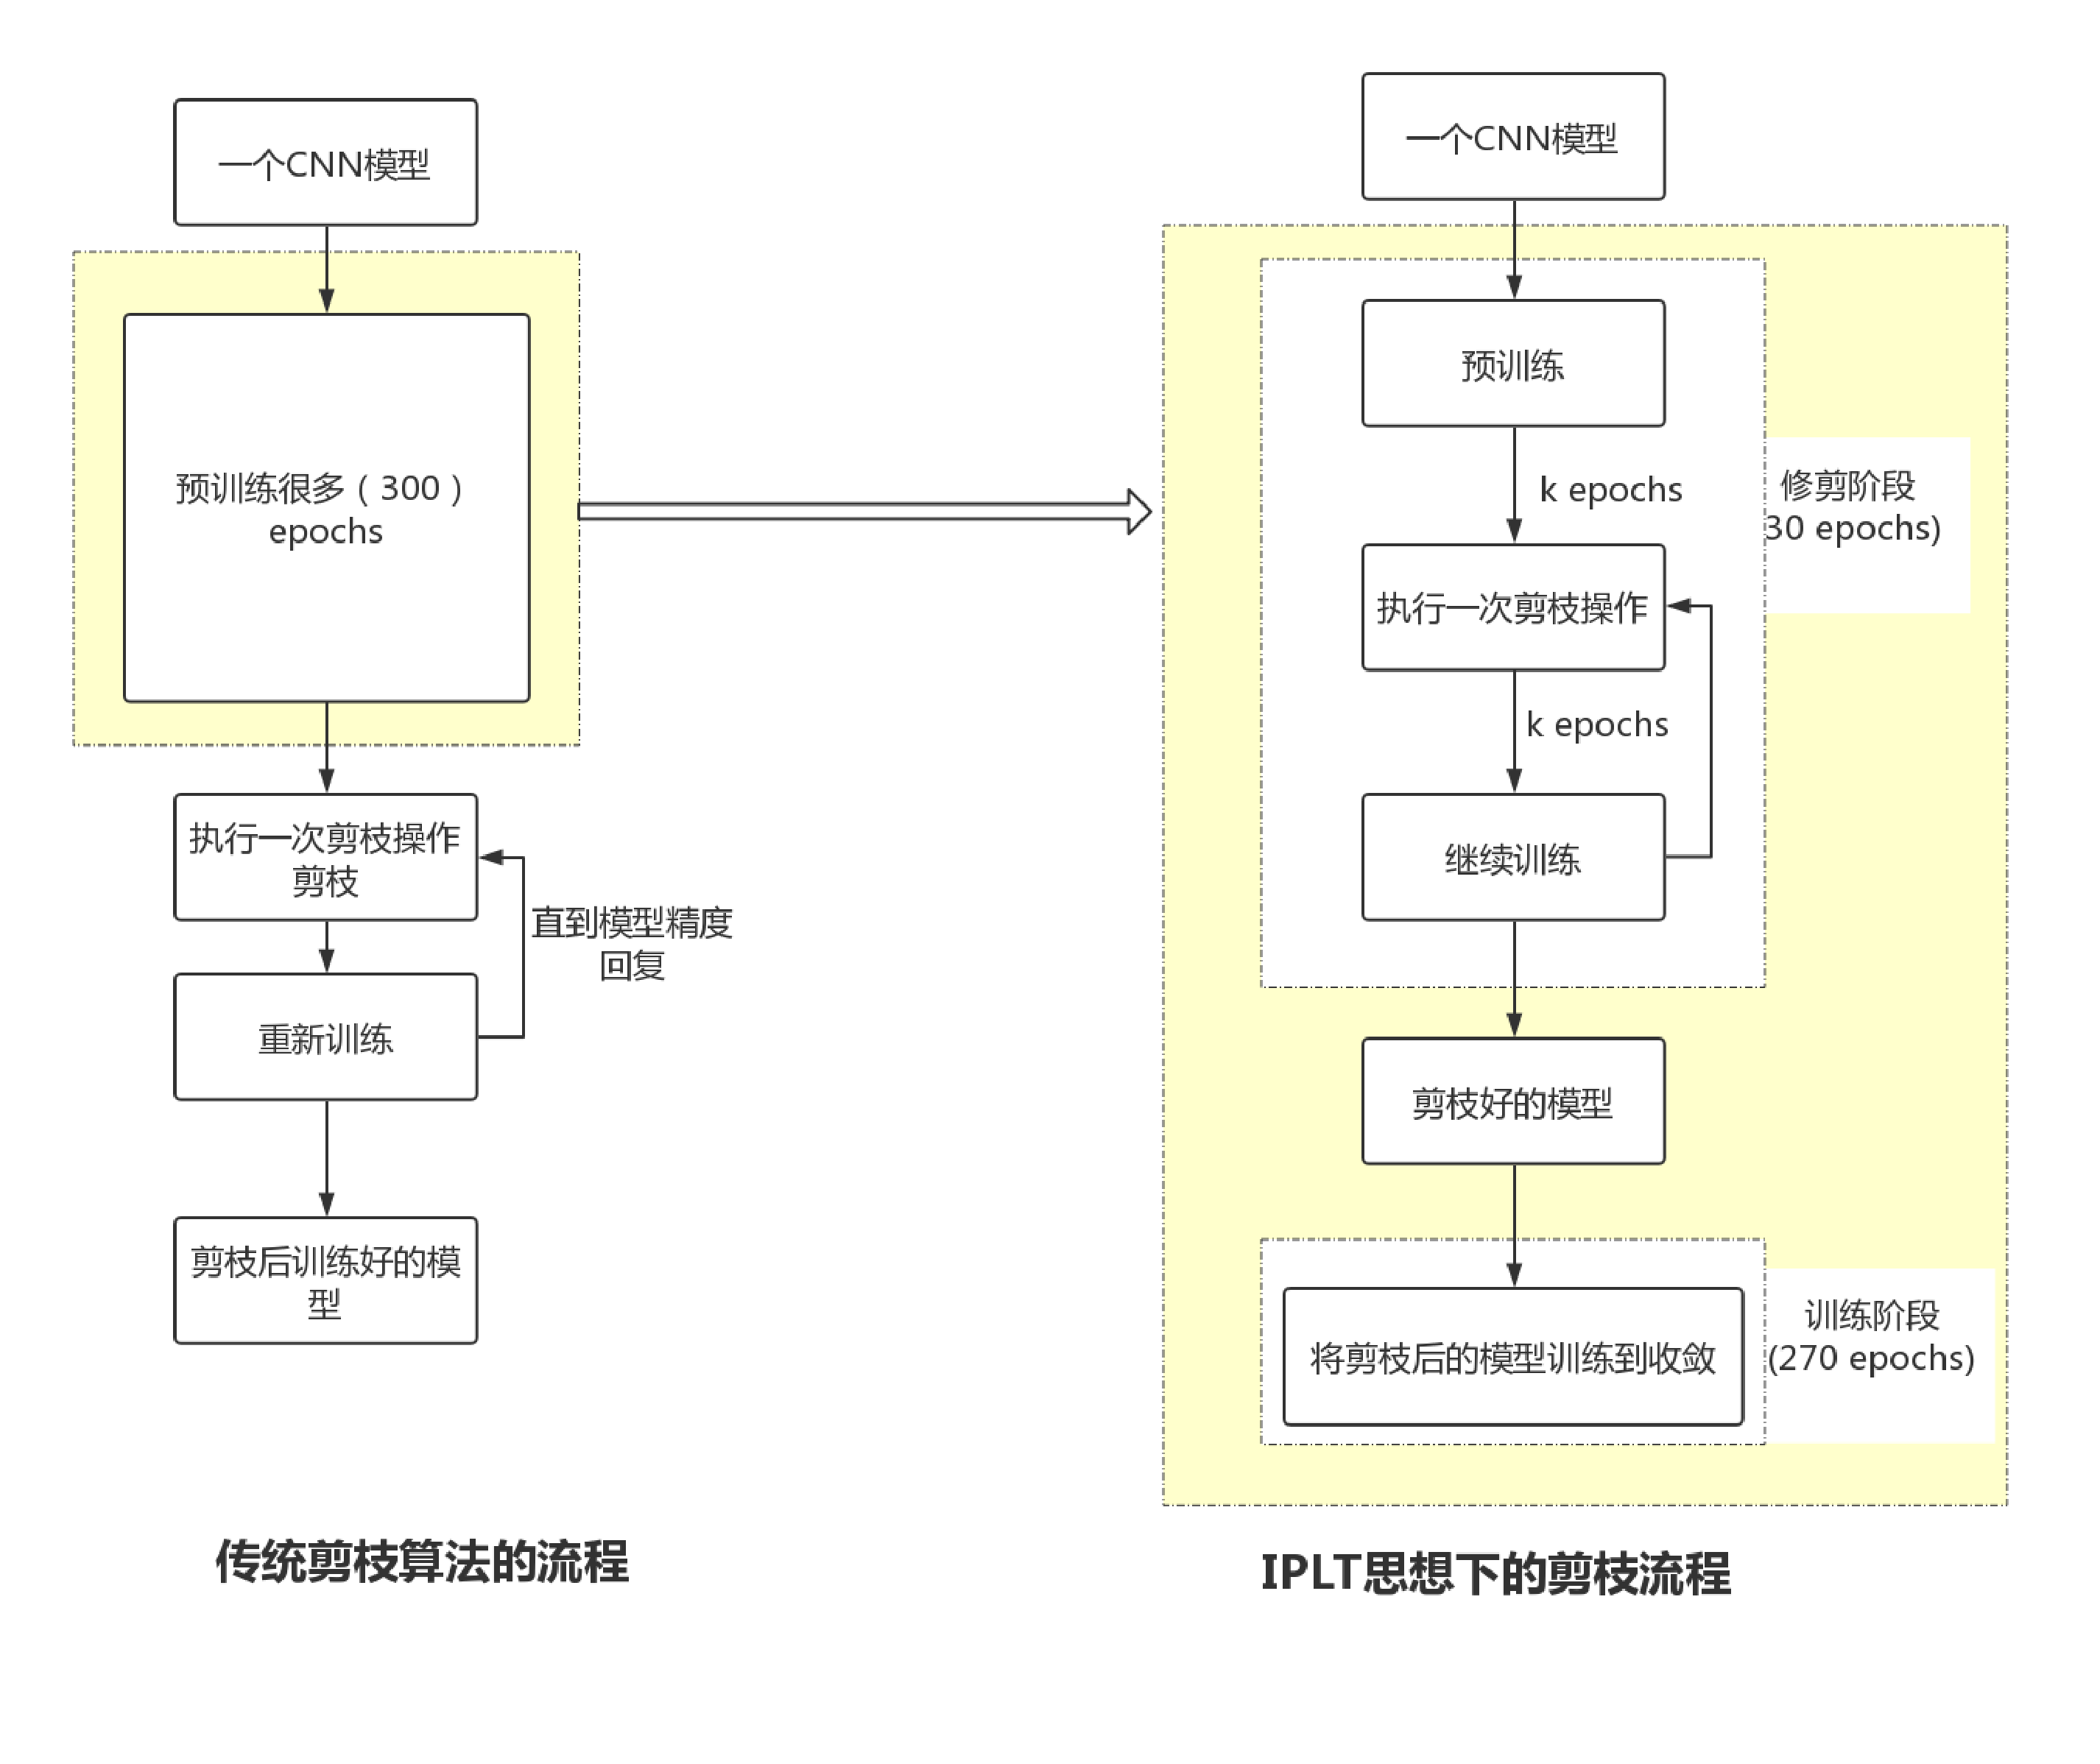
\includegraphics[width=\textwidth]{pruning_contrast.pdf}
\caption{传统剪枝思想和IPLT剪枝思想的对比}
\label{pruning_contrast2}
\end{figure}

图 \ref{pruning_contrast2}中左侧是传统剪枝算法的流程,右侧是IPLT剪枝思想的流程。图中黄色部分表示的是300epochs的训练。传统剪枝算法中,经过200epochs才训练出来一个预训练好的模型,但是还需要迭代剪枝,重训练(retrain)很多周期才能得到一个剪枝好、可使用的模型。而在右侧,同样是300epochs,前30epochs内,IPLT已经完成了对模型的剪枝,在之后的270个epochs中一直训练的是一个剪完枝的CNN模型。不仅300epochs就得到了一个剪完枝的、可使用的模型;同时在后270epochs的训练中,训练算法一直训练的是一个精简后的模型,这样的模型在训练中计算消耗更少——前向、反向计算消耗都小!

在IPLT思想中,首先需要确定一个超参k,我在训练模型的过程中将每隔k个epochs就进行一次剪枝,假定k值被设定为5。其次需要确定一个剪枝比例序列,如$\{10\%, 20\%, 30\%, \dots, 80\%,\}$。那么意味着,一个随机初始化的模型,剪枝算法会在第5、10、15、···、40个周期的训练结束后各执行一次剪枝操作。第一次剪枝操作,剪去整个网络10\%的filters;第二次剪枝要修剪整个网络20\%的filters,因为第一次剪枝已经剪去10\%,所以只需要额外再剪去10\%的filters即可;同理,第三次剪枝需要再剪去额外的10\%的filters;以此类推。最终前40个epochs中,剪枝算法将共执行剪枝操作8次,最终将CNN模型80\%的filters剪去。

在之后的训练中,因为算法已经完成了剪枝操作,所以只需要对剩下20\%filters的CNN模型执行正常训练即可。因为此时模型只剩下20\%的filters,所以显然不论是前向运算还是反向求每个参数的梯度时的计算量,都比训练完整模型时小多了。因此IPLT思想能优化网络训练过程的计算量。IPLT改进之后的剪枝算法是目前唯一一类能优化预训练过程的的剪枝算法。

\subsection{基于IPLT思想改进的经典剪枝算法}

本章基于IPLT思想对\cite{17}中的算法进行了改进。改进后的算法流程如算法.\ref{17iplt}

\begin{algorithm}[htb]
  \caption{\cite{17}中剪枝算法基于IPLT思想改进后流程}
  \label{17iplt}
  \begin{algorithmic}[1]
    \REQUIRE
      训练集:X, 训练最大周期数: $epoch_{max}$,
      增量式剪枝比例序列: $L = \left\{R_1, R_2, ..., R_n\right\}$ ,
      网络参数: $\mathcal{W} = \left\{\mathcal{W}_i , 1\leq i \leq L \right\}$,
      一个CNN模型, ${W_l,1\leq l\leq L}$;\\
    \ENSURE 模型第L层的参数为:${\hat{W_l}, 1\leq l\leq L}$;
    \STATE 初始化模型参数: ${W_l}$, ${1\leq l\leq L}$ ;超参数: k;ind=0;
    \STATE 对于 ${epoch=1, 2, \ldots, epoch_{max}}$, 执行:
    \STATE \qquad 如果 epoch\%k==0 且 $ind<len(L)$:
    \STATE \qquad \qquad 对于 $i=0, 1, \ldots, L$, 执行:
    \STATE \qquad \qquad \qquad 根据$l2$范数的计算方法,计算每个filter $\mathcal{F}_{i,j}, 1\leq j \leq I_i$ 的重要性;

    \STATE \qquad \qquad  根绝global模式,将所有filters重要性排序,并剪去 $R_{ind}\ast\sum_{i=1}^LO_i$;
    \STATE \qquad \qquad ind = ind+1
    \STATE \qquad 根据训练集$X$,训练模型,更新网络参数 $W$;
    \STATE Return 剪枝完,训练完的模型;
  \end{algorithmic}
\end{algorithm}

改进后的经典剪枝算法不需要再将模型训练到收敛,而是初始化模型之后开始,间隔k个训练周期就将模型剪枝一次。剪filters时,对filters的重要性度量方法和\cite{17}相同,采用$l2$范数作为filters重要性的衡量标准。在剪枝时,改进后的经典剪枝算法依然选择了global模式的比较模式,整个网络所有filters一起比较重要性。

%%%%%%%%%%

\subsection{基于IPLT思想改进的Soft剪枝算法}

本章基于IPLT思想对\cite{27}中的算法进行了改进。改进后的算法流程如算法.\ref{27iplt}

\begin{algorithm}[htb]
  \caption{\cite{27}中剪枝算法基于IPLT思想改进后流程}
  \label{27iplt}
  \begin{algorithmic}[1]
    \REQUIRE
      训练集:X, 训练最大周期数: $epoch_{max}$,
      增量式剪枝比例序列: $L = \left\{R_1, R_2, ..., R_n\right\}$ ,
      网络参数: $\mathcal{W} = \left\{\mathcal{W}_i , 1\leq i \leq L \right\}$,
      一个CNN模型, ${W_l,1\leq l\leq L}$;\\
    \ENSURE 模型第L层的参数为:${\hat{W_l}, 1\leq l\leq L}$;
    \STATE 初始化模型参数: ${W_l}$, ${1\leq l\leq L}$ ;超参数: k;ind=0;
    \STATE 对于 ${epoch=1, 2, \ldots, epoch_{max}}$, 执行:
    \STATE \qquad 如果 epoch\%k==0 且 $ind<len(L)$:
    \STATE \qquad \qquad 对于 $i=0, 1, \ldots, L$, 执行:
    \STATE \qquad \qquad \qquad 根据$l2$范数的计算方法,计算每个filter $\mathcal{F}_{i,j}, 1\leq j \leq I_i$ 的重要性;

    \STATE \qquad \qquad  根绝global模式,将所有filters重要性排序,将 $R_{ind}\ast\sum_{i=1}^LO_i$个filters参数设为0;

    \STATE \qquad \qquad 如果ind==Len(L)-1:
    \STATE \qquad \qquad \qquad 将 $R_{ind}\ast\sum_{i=1}^LO_i$个filters实际剪去

    \STATE \qquad \qquad ind = ind+1
    \STATE \qquad 根据训练集$X$,训练模型,更新网络参数 $W$;
    \STATE Return 剪枝完,训练完的模型;
  \end{algorithmic}
\end{algorithm}

改进后的Soft剪枝算法采用了和原算法\cite{27}相同的filters重要性度量标准,即公式 \ref{l2},fiters的$l2$范数。原算法中,每个epoch的训练之后,都会对网络中filters进行一次Soft剪枝。改进的算法中也保留了该机制。

首先,改进后的Soft剪枝依然不需要再将模型训练到收敛,而是间隔一定个周期就将模型剪枝一次。这点上,改进前后的算法是一致的。因为\cite{27}中算法选定的剪枝间隔epoch数是1,所以本文将IPLT改进后的剪枝算法中执行剪枝操作的间隔(必须强调,这不是IPLT思想中的k值)也设定为1。

本文在IPLT思想中提出,基于少量训练后执行剪枝操作时,如果一次性修剪过高比例,容易影响剪枝后模型的精度,所以引入了增量式的剪枝思想。而在\cite{27}中,每次剪枝的比例都是恒定的,每次剪枝都采用了相同的剪枝比例$tr$(假设目标剪枝比例为$80\%$)。本章在改进后的Soft剪枝算法中,将剪比例恒定这点做了调整,根据增量式的思想,本章依然采取了逐步提高剪枝比例的做法。在改进后的Soft剪枝算法中,需要设定了一个剪枝比例序列,如$\{10\%, 20\%, 30\%, \dots, 80\%\}$。在IPLT思想中有一个超参数k,原来k值指的是隔k个周期剪枝一次。因为\cite{27}中是每个epoch之后都要执行剪枝操作的,所以在改进后的软算法中k值的含义被稍作修改。基于IPLT思想改进后的Soft剪枝算法中,这个k是指隔k个epochs改变一次剪枝操作的比例。以上述剪枝比例序列$\{10\%, 20\%, 30\%, \dots, 80\%\}$为例,假定k值取为5。在执行剪枝算法的时候,前5个epoch每个epoch的训练完毕之后,改进后的Soft剪枝算法都会执行一次Soft剪枝操作,并且这五次Soft剪枝操作的剪枝比例都是$10\%$;在第6个epoch的训练之后(已经过了5个epochs),剪枝操作的剪枝比例调整为$20\%$。在第6至第10个epoch的训练之后的剪枝操作中,剪枝比例始终为$20\%$;在第11个epoch的训练之后(又过了5个epochs),剪枝操作的剪枝比例调整为$30\%$。在第11至第15个epoch的训练之后的剪枝操作中,剪枝比例始终为$30\%$··· 以此类推,最后在第35至第40个epoch的训练之后的剪枝操作中,剪枝比例始终为$80\%$。在第40个epoch时,所有的剪枝操作执行完毕。在第41个epoch之后,只执行对网络的训练,不再执行对网络的剪枝操作。

在剪枝filters时,需要对filters重要性度量。为了保证对比实验的说服力,改进后Soft剪枝算法中对filters的重要性度量方法和\cite{27}相同,采用$l2$范数作为filters重要性的衡量标准。\cite{27}中对filters重要性进行排序时,选择的是intra-layer模式,因此改进后的Soft剪枝算法也选择了intra-layer模式的比较模式,将CNN网络各层内filters各自进行排序,比较重要性,每次剪枝操作各层按照剪枝比例剪去相同比例的filters。

\section{实验设定}

\subsection{数据集和模型选定}

本实验数据集选定了MNIST,CIFAR10数据集。验证模型选择VGGNet和ResNet。MNIST数据集已经在上一个章节中做了介绍,本节详细介绍一下CIFAR10数据集。CIFAR10数据集是一个彩色图片数据集,每张图片都是RGB三通道,图片大小为$32*32$像素。CIFAR10数据集共有十个类别,本章将这十个类别的图片打印,展示在了图 \ref{cifar10_dataset}中。彩色图像存储原理和黑白图像类似,但是一张黑白图像只需要存储一个矩阵即可,而彩色图像则需要存储三个矩阵。这三个矩阵分别对应红、绿、蓝三种颜色。这三个矩阵中存储了0-255的数字,每个数字对应一个像素点,数字越大表明该像素点颜色越深。红、绿、蓝三张图片叠加出来的就是日常生活中看到的彩色图片。

\begin{figure}
\centering
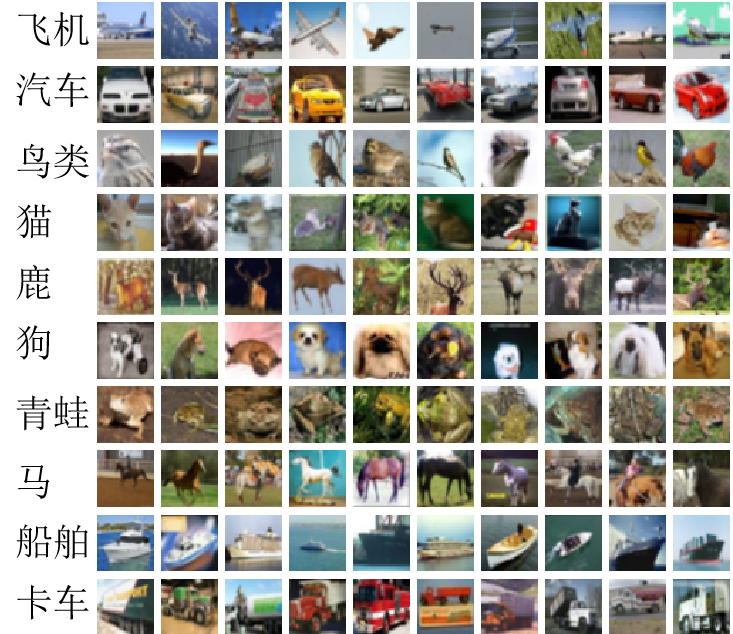
\includegraphics[width=\textwidth]{cifar10.png}
\caption{CIFAR10数据集中图片展示}
\label{cifar10_dataset}
\end{figure}

实验验证模型分别选择了一个普通的CNN模型,VGG19模型以及ResNet模型。

\subsection{剪枝算法实现方案}

现有的剪枝算法,在实现时共有两种方案。第一种可以称之为“虚拟剪枝”,这种剪枝方法只是在效果上等价于剪枝。实际实现时是通过添加mask实现。即对应于每个filter,构造一个相同大小的mask。该mask有0、1组成:如果某个filter被剪去,则mask中对应位置全部设置为0,如果filters没有被剪去,则mask中对应位置全部设置为1。在执行卷积操作前,参数先和mask做一次乘法,这样被剪去的filters中不论参数如何,都会在乘法操作之后变成0;然后用乘出来的参数执行卷积操作,最终这部分被剪去的filters在效果上等价于被剪去了。第二种可以称之为“真实剪枝”,这种剪枝方法是真实将网络剪枝了。一般这种算法的在执行剪枝操作时,都是生成一个新的CNN网络,这个新的网络形状和剪枝后的网络形状相同。然后将应该保留的、未被剪去的参数复制到这个新的模型中。之后不管是retraining操作还是剪枝操作都是对这个新的模型进行。

在\cite{17}中作者并没有表明如何实现剪枝策略,因此本章在复现\cite{17}和实现其改进算法的时候选择了第二种实现方法,“真实剪枝”的策略。而在\cite{27}中,由于作者本身是基于“虚拟剪枝”的剪枝策略实现的Soft剪枝算法,为了便于比较本章也基于该剪枝策略实现了改进的Soft剪枝算法。

\section{实验结果及分析} \label{2result}

\subsection{实验对比策略}

基于传统的剪枝思想的剪枝算法,在执行剪枝操作之前会基于完整的模型训练出一个收敛的模型。然后基于这个预训练好的模型执行剪枝策略。而基于IPLT剪枝思想的剪枝策略,是在训练初期就完成剪枝的,所以基于IPLT思想执行剪枝操作的时候,是不会得到完整模型的分类精度的。为了保证能够有效对比原始剪枝策略和基于IPLT改进后剪枝策略的效果,本章实验将记录并对比三个数据:1.预训练的完整CNN模型的测试精度;2.基于传统剪枝策略,对预训练模型剪枝后的测试精度;3.基于IPLT改进的剪枝策略,训练出来的剪枝后模型的测试精度。

在对比传统剪枝策略和基于IPLT改进后剪枝策略时,不论是哪种剪枝策略,首先需要保证剪枝后模型的精度不受影响。即剪枝后模型的精度不应明显低于完整模型在同一数据集上的精度。基于CNN、MNIST数据集的剪枝对比实验,将选择保证剪枝后网络的精度,对比filters剪枝比例(存储空间的优化)。测试精度相似,而最大filters剪枝比例相近则说明两类剪枝策略在剪枝效果上差异不大,若某种剪枝策略能在保证模型精度的前提下剪掉更多的filters则说明该剪枝策略剪枝效果更好。基于CIFAR10剪枝VGG16和ResNet的对比实验,将在保证模型精度的前提下,对比对模型前向计算中被剪去的计算量(计算量优化)。一般来说,剪去的filters越多,在前向计算时,该模型所需要完成的计算量就越少(被剪去的计算量的比例就越大)。

\subsection{原经典剪枝算法VS基于IPLT改进的经典剪枝算法} \label{norm_pruning}

基于MNIST数据集和一个普通的CNN网络,实验中对比了\cite{17}中的经典剪枝策略以及基于IPLT思想改进的经典剪枝策略的剪枝效果。实验设置上,因为MNIST数据集复杂度相对较低,因此超参k设置为2。filters剪枝比例序列为类似$\{10\%, 20\%, \dots, 60\%, 65\%\}$的形式,除了最后一次的剪枝比例为目标剪枝比例,之前每次剪枝都比上次多剪去$10\%$的filters。实验结果如下表 \ref{2mnist}

\begin{table}[!htbp]
\caption{基于MNIST数据集和CNN模型,经典剪枝算法改进前后的效果对比}
\begin{tabular}{|c|c|c|c|}
\hline
{Mode} & {$FPR_{all}$} & $PPR_{all}$ & $Accuracy(\%)$ \\ \hline
baseline & 0.00 & 0.00 & 99.35 \\ \hline
$original\_pruning$ & 60.00 & 83.05 & 99.32 \\
$original\_pruning$  & 65.00 & 83.05 & 99.36 \\
$original\_pruning$  & 70.00 & 90.65 & 99.17 \\ \hline
$modified\_pruning$  & 60.00 & 84.72 & 99.35\\
$modified\_pruning$ & 65.00 & 87.89 & 99.31\\
$modified\_pruning$ & 70.00 & 95.47 & 99.28\\ \hline
\end{tabular}
\label{2mnist}
\end{table}

表格中,baseline指的是预训练的完整模型。$original\_pruning$是指的原经典剪枝策略\cite{17}。$modified\_pruning$指的是基于IPLT思想改进的经典剪枝策略。表格中$FPR_{all}$指的是最终CNN网络中filters被剪去的数量占全部filters数量的比例。$PPR_{all}$指的是整个网络被剪去的参数个数占总参数个数的比例。$Accuracy$指的是测试精度,单位是$\%$。

该CNN模型在MNIST数据集上训练出来的测试精度为$99.35\%$。之后基于改进前后两种经典剪枝策略,按照$60\%$,$65\%$,$70\%$三种filters剪枝比例进行了剪枝实验。从表 \ref{2mnist}中可以看到,在filters剪枝比例相同的前提下,基于\cite{17}中的经典剪枝策略和基于IPLT思想改进后的剪枝策略,剪完的CNN模型测试在测试精度上并没有太大的差异。即在MNIST数据集和CNN模型上,基于少量预训练和基于大量预训练,最终剪枝效果上并没有太大的差异。

基于CIFAR10数据集和VGG16网络,本段的实验对比了\cite{17}中的经典剪枝策略以及基于IPLT思想改进的经典剪枝策略。实验设置上,因为CIFAR10数据集复杂度相对较高,因此超参k被设置为5。filters剪枝比例序列为类似

$\{10\%, 20\%, 30\%, \dots, 60\%, 65\%\}$

\noindent 的形式,除了最后一次的剪枝比例为目标剪枝比例,之前每次剪枝都比上次多剪去$10\%$的filters。实验结果如下表 \ref{2cifarvgg}。

\begin{table}[htbp]
 \caption{基于CIFAR10数据集和VGG16,经典剪枝算法改进前后的效果对比}
 \begin{tabular}{cccccc}
  \hline
  Model&$FPR$&Model Size(MB)&FLOPs&Pruned FLOPs(\%)&Accuracy(\%)\\
  \hline
  \hline
  original baseline&-&-&$3.13 \times 10^8$&0.00&93.25\\
  \hline
  $original\_pruning$&-&-&$2.06 \times 10^8$&34.20&93.40\\
  \hline
  $our\_baseline$&0.00&58.9&$3.13 \times 10^8$&0.00&94.33\\
  \hline
  \textbf{$modified\_pruning$}&60&9.7&$1.52 \times 10^8$&51.36&94.35\\
  \textbf{$modified\_pruning$}&70&6.0&$1.27 \times 10^8$&59.54&94.05\\
  \hline
 \end{tabular}
\label{2cifarvgg}
\end{table}

该实验中部分结果引用自\cite{17},所以有两个baseline。表格中,original baseline指的是\cite{17}中预训练的完整模型的精度。$our\_baseline$指的是复现的完整的VGG16模型,在CIFAR10数据集上训练后的测试精度。$original\_pruning$是指的原经典剪枝策略\cite{17}。$modified\_pruning$指的是基于IPLT思想改进的经典剪枝策略。表格中$FPR_{all}$指的是CNN网络中最终filters被剪去的比例。Model Size指的是基于pytorch库,保存了模型,记录下的模型的存储大小,单位是MB。FLOPs指的是,模型在执行一次前向计算的时候需要做多少浮点数运算(计算消耗)。Pruned FLOPs指的是通过剪枝算法剪枝后的模型在执行前向计算时,浮点数计算量相较于完整模型前向计算时的计算量,少了多少,单位是$\%$。$Accuracy$指的是测试精度,单位是$\%$。

\cite{17}原文中VGG16模型在CIFAR10数据集上训练出来的测试精度为$93.25\%$,在同样情况下训练VGG16模型得到的精度为$94.33\%$。\cite{17}中记录了原经典剪枝算法在保证模型精度的前提下,最多能将模型前向计算中$34.20\%$的计算量剪去。基于IPLT思想改进了经典剪枝策略,按照$60\%$,$70\%$两种filters剪枝比例进行了剪枝实验。从表 \ref{2mnist}中最下面两行可以看出,当filters剪枝比例为$60\%$时,此时剪枝后模型精度不仅没有损失还略有上升,同时前向计算的计算量优化比例为$51.36\%$远远高于原始的\cite{17}中的计算量优化比例。可见基于IPLT思想优化后的经典剪枝策略,在模型计算量优化方面性能完全不输于原始的\cite{17}的范数优化策略。



\subsection{Soft剪枝VS基于IPLT改进的Soft剪枝}

基于CIFAR10数据集和ResNet-110网络,本章对比了\cite{27}中的Soft剪枝策略以及基于IPLT思想改进后的Soft剪枝策略。表 \ref{2cifarresnet}中一部分数据来自原文\cite{27}。同时本章也复现了原Soft剪枝算法,并实现了改进的Soft剪枝算法,记录了实验结果。实验设置上,因为CIFAR10数据集复杂度相对较高,因此超参k被设置为5。filters剪枝比例序列为类似$\{10\%, 20\%, 30\%, \dots, 60\%\}$的形式,每次调整剪枝比例都比上一次多剪去$10\%$的filters。实验结果如下表 \ref{2cifarresnet}。

\begin{table}[htbp]
 \caption{基于CIFAR10数据集和ResNet-110模型,Soft剪枝算法改进前后效果对比}
 \begin{tabular}{cccccc}
  \hline
  \hline
  Model&$FPR$&Model Size(MB)&FLOPs&Pruned FLOPs(\%)&Accuracy(\%)\\

  \hline
  paper's baseline&0.00&-&-&-&94.00\\
  \hline
  original in paper&10&-&$2.16 \times 10^8$&14.60&94.02\\
  original in paper&20&-&$1.82 \times 10^8$&28.20&94.34\\
  original in paper&30&-&$1.50 \times 10^8$&40.80&93.68\\
  \hline
  \hline
  $our\_baseline$&0.00&-&$3.9 \times 10^8$&0.00&95.17\\
  \hline
  our original&10&-&$2.16 \times 10^8$&14.60&95.07\\
  our original&20&-&$1.82 \times 10^8$&28.20&94.89\\
  our original&30&-&$1.50 \times 10^8$&40.80&94.93\\
  \hline
  our modified&10&-&$2.16 \times 10^8$&14.60&95.18\\
  our modified&20&-&$1.82 \times 10^8$&28.20&95.09\\
  our modified&30&-&$1.50 \times 10^8$&40.80&94.96\\

  \hline
  \hline
 \end{tabular}
\label{2cifarresnet}
\end{table}

该实验中部分结果引用自\cite{27},由于本章也复现了原文的算法,所以有两个baseline。表格中,paper's baseline指的是原文\cite{27}中作者基于CIFAR10数据集,训练ResNet-110完整模型得到的精度为$94.00\%$。$our\_baseline$指的是复现后完整的ResNet-110模型,在CIFAR10数据集上训练得到的精度为$95.17\%$。表格中original in paper指的是,原始的Soft剪枝策略;our original指的是复现后的原Soft剪枝策略剪枝后模型的测试精度(original指的是原始剪枝策略,这里指的是Soft剪枝)。our modified指的是本章复现的基于IPLT思想改进后的Soft剪枝策略剪枝后模型的测试精度。表格中$FPR_{all}$指的是CNN网络中最终filters被剪去的比例。Model Size指的是基于Pytorch库,保存了模型,记录下的模型的存储大小,单位是MB。但是由于文\cite{27}是“虚拟剪枝”,所以表格中并没有能存下有效的基于Pytorch库中的模型存储大小。FLOPs指的是,模型在执行一次前向计算的时候需要做多少浮点数运算(计算消耗)。Pruned FLOPs指的是通过剪枝算法剪枝后的模型在执行前向计算时,浮点数计算量相较于完整模型前向计算时的计算量,少了多少,单位是$\%$。$Accuracy$指的是测试精度,单位是$\%$。

\cite{27}原文中ResNet-110模型在CIFAR10数据集上训练出来的测试精度为$94.00\%$,本章在同样情况下训练ResNet-110模型得到的精度为$94.33\%$。\cite{27}中记录了原Soft剪枝算法在保证模型精度的前提下,最多能将模型中$20\%$的filters剪去,前向计算中$28.20\%$的计算量剪去。本章复现的Soft剪枝策略,在剪枝时效果与原文基本相同;只是原文中$FPR_{all}$设定为$20\%$时,网络精度反而有一定提升;而本章复现的Soft剪枝策略中,$FPR_{all}$设定为$20\%$时,网络精度有小幅下降。基于控制变量法原则,对比实验结果应当以本文复现结果对比,更有说服力。

本章实现的两个版本的Soft剪枝策略(原始Soft剪枝策略和改进的Soft剪枝策略)中,设定$FPR_{all}$为$10\%$时,都不会影响模型的精度。在改进的Soft剪枝策略中,设定$FPR_{all}$为$20\%$时,模型测试精度只有小幅下降,且下降幅度比原Soft剪枝策略低。可见在$FPR_ {all}$设定为$20\%$的情况下,基于IPLT改进的Soft剪枝策略相较于原始Soft剪枝策略,剪枝操作对模型精度的影响更小。当$FPR_ {all}$设定为$30\%$的情况下,改进前后的Soft剪枝策略都造成了模型精度的下降,且下降幅度相近(分别$0.24\%$和$0.21\%$)。因为\cite{27}和本文复现Soft剪枝算法时,对filters重要性的排序都是基于intra-layer模式,所以$FPR_ {all}$设定相同的情况下,$Pruned FLOPs$是相同的,即在本次对比实验中,剪枝相同比例的filters。因为是intra-layer模式,所以剪枝算法不仅对模型的存储压缩效果相同,对模型前向计算时计算量的优化效果也相同。

通过以上对比及说明,本文可以发现,基于IPLT改进的Soft剪枝策略在模型压缩相同存储空间,优化相同计算量比例的情况下,剪枝精度是完全不弱于原始Soft剪枝策略的。即基于IPLT改进的Soft剪枝策略至少在剪枝效果上是不弱于原始Soft剪枝策略的。

\section{本章小结}

在第 \ref{2result}章节中,我们利用IPLT思想改造了现有的两个剪枝策略:1.经典剪枝策略\cite{17};2.Soft剪枝策略\cite{27}。在第 \ref{2result}章节中也对比,并说明了对比结果。数据数据说明,在保证CNN模型精度的前提下,基于IPLT思想改进的剪枝策略能实现更高至少是相近的模型存储压缩比例、计算量优化比例。可见,在剪枝效果上,基于IPLT思想改进的剪枝策略是不弱于原始剪枝策略的。

我们必须强调基于IPLT思想改进的剪枝策略另一优势,如图 \ref{pruning_contrast2}中所表现出来的,IPLT改进的剪枝策略,在前几十个epochs就将模型剪枝完毕,所以在之后的训练过程中一直训练的是一个精简后的模型。基于IPLT改进的剪枝策略在CNN模型训练阶段(相当于图 \ref{pruning_contrast2}中所述,左边的传统剪枝算法中的预训练阶段或者右边的IPLT思想中的训练阶段),对模型进行训练时的计算量要大大降低。

为了进一步证明基于IPLT确实能优化模型训练过程的计算消耗,实验时我们记录了一组第 \ref{norm_pruning}章节中经典剪枝改进前后的训练时间。实验中设定,训练周期数为300epochs,先训练了一个完整VGG16模型,共耗时7253.6323s;之后测试了利用改进后的经典剪枝\cite{17}算法对VGG16进行剪枝,前30个epchs完成剪枝,又训练了70epochs,一共训练了300epochs,耗时共5319.2427s。这组实验耗时记录上虽然不能准确反应IPLT思想对剪枝算法的模型训练阶段计算量的优化幅度,但是从时间上可以明显看出IPLT思想对模型的训练阶段是有优化效果的。


1.IPLT思想在性能上的优势:基于IPLT思想改进了两个现有的剪枝策略。这两个剪枝策略剪枝后的性能都不弱于剪枝前,且剪枝后算法在模型训练过程中的计算消耗也被大大优化。
2.IPLT思想的可行性:通过第 \ref{2result}章节中的对比实验,证明了IPLT思想至少能来优化经典剪枝策略\cite{17}和\cite{27}。这无疑证明了基于IPLT思想的改进至少对部分剪枝策略是可行的。


\chapter{总结与展望}

\section{工作总结}

深度学习算法由于其性能优势,近年来如图像识别、图像描述生成、自然语言处理等领域取得了广泛的应用。但深度学习模型高精度的同时,往往模型存储空间占有大、应用时计算量大。对硬件存储和计算性能的高要求,限制了深度学习算法的广泛应用。大量的研究者开始将目标转向对深度学习模型压缩、加速的研究上。其中对卷积神经网络(CNN)的压缩、加速是近年来的研究热门。我们的研究工作也集中于对CNN模型的压缩、加速。

现有对深度学习模型压缩、加速的算法大致分为三类:量化、剪枝和模型轻量化。本文的三项工作主要集中于对量化、剪枝算法的思考、改进。

1.大量的研究者尝试不同的算法思路,在保证模型精度的前提下,实现对CNN更好的量化效果——参数比特位更少,计算优化更好。但我们发现,现有的量化算法的目标值往往是基于直觉,很少有研究者对量化算法的量化目标值进行研究。一个高效的量化目标值集合,能以更少的数值,拟合原来的全精度网络。因此本文第一项工作中尝试根据CNN网络参数的分布,优化量化目标值集合。最终实验结果证明:基于相同的量化策略,在保证模型精度的前提下,优化之后的量化目标值集合需要的参数更少。即,通过对量化目标值集合的优化,可以进一步压缩表示一个参数所需要的bit位数,基于相同的量化算法,能实现对CNN模型存储更好的压缩效果。

2.现有的量化算法,总是整个网络或者整个卷积层共用一个量化目标值集合。在量化目标集合包含数值较多的情况下,这种以网络、卷积层为量化集合应用范围的思路不会影响量化之后模型的精度。但是当量化算法希望将模型存储尽可能压缩时,如极限的二值化\cite{binary}、三值化\cite{ternary}时,整个网络或者一个卷积层共用相同量化目标值集合,无疑会影响最终模型的精度。

针对这一问题,我们本文第二项工作中提出了调整量化目标值集合应用范围的思路,针对卷积网络中各个filters生成相应的量化目标值。对比实验中,通过对不同的filters生成特定的量化目标值,在模型压缩效果和计算优化效果不变的情况下,量化之后模型能取得更高的测试精度。证明了改变量化目标值应用范围,这一思路的有效性。

3.现有剪枝算法总是基于大量的预训练。然而大量的预训练意味着大量的计算资源的消耗。我们本文第三项工作提出了基于少量预训练的剪枝思想,并利用该思想改进了\cite{17}和\cite{27}。通过实验发现基于少量预训练,现有的部分剪枝算法依然能实现很好的剪枝性能。基于少量训练就完成剪枝操作,能大大优化模型训练阶段消耗的计算资源。


\section{研究展望}
1.本文中,我们只是针对filters生成了对应的量化目标值集合。事实上还可以尝试对其他单位的参数,生成对应的量化目标值集合。如针对filters中的某部分参数生成特定的量化集合。

2.本文中,通过对比实验,我们证明了基于少量预训练的剪枝思想的可行性。但是还有两方面的工作值得进一步研究:(1).现有的剪枝算法是否都能用基于少量训练的剪枝算法改进;(2).基于少量预训练的剪枝思想中,少量预训练到底少到什么程度是最佳的。预训练的epochs数目,到底依赖模型本身还是数据集的复杂度。


%######################



%%%%%%%%%%%%%%%%%%%%%%%%%%%%%%
%% 附件部分
%%%%%%%%%%%%%%%%%%%%%%%%%%%%%%
\backmatter

% 参考文献
% 使用 BibTeX,不使用 BibTeX 时注释掉下面一句。
\bibliography{template}

% 不使用 BibTeX
%\begin{thebibliography}{2}
%
%\bibitem{deng:01a}
%{邓建松,~彭冉冉,~陈长松}.
%\newblock {\em \LaTeXe{}~科技排版指南}.
%\newblock 科学出版社,~书号:~7-03-009239-2/TP.1516, 北京, 2001.
%
%\bibitem{wang:00a}
%王磊.
%\newblock {\em \LaTeXe{}~插图指南}.
%\newblock 2000.
%\end{thebibliography}

% 本章可以删去



  % 致谢
\begin{thanks}
\vskip 18pt

%首先感谢XXX

\end{thanks}


\end{document}
